\documentclass[12pt,a4paper,twoside]{stb}

\usepackage{cmap}
\usepackage[T2A]{fontenc}
\usepackage[utf8]{inputenc}
\usepackage[english,russian]{babel}

\usepackage{amsmath,amssymb,xspace,xifthen,graphicx,float,color}
\usepackage{ucs,textcase,verbatim}

\usepackage[
  pdftitle={Encryption and Integrity Control Algorithms},
  pdfauthor={},
  pdfpagemode=UseOutlines,
  pdfstartview=FitH,
  linkcolor=black,
  citecolor=black]{hyperref}

\usepackage{ulem}
\normalem

\usepackage{longtable}
\setlongtables

\usepackage{enumitem}
\setlist[1]{itemsep=0pt,parsep=0pt,topsep=0pt,partopsep=0pt,
  align=left,
  leftmargin=0pt,itemindent=1.6\parindent,
  labelindent=\parindent,labelwidth=0.5\parindent,labelsep=*,
  listparindent=\parindent}
\setlist[2]{itemsep=0pt,parsep=0pt,topsep=0pt,partopsep=0pt,
  leftmargin=2.4\parindent}
\setlist[enumerate,1]{label=\arabic*}
\setlist[enumerate,2]{label=\arabic*)}
\setlist[itemize,1]{label=--}

\usepackage{_defs}

\setcounter{tocdepth}{1}
\pagestyle{headings}

\hoffset          = -1in 
\voffset          = -1in
\oddsidemargin    = 30mm             % стандарт ТКП 1.5-2004            
\evensidemargin   = 10mm             % верхнее = 20 мм                  
\textwidth        = 170mm            % правое  = 10 мм                  
\topmargin        = 20mm             % левое и нижнее = не менее 20 мм  
\textheight       = 252mm  
\headsep          = 1\baselineskip
\headheight       = 2\baselineskip
\addtolength{\topmargin}{-\headheight}
\addtolength{\topmargin}{-\headsep}
\parindent        = 0.8cm
\intextsep        = 3pt

\renewcommand{\baselinestretch}{1.015}
\setcounter{tocdepth}{1}

\begin{document}
\begin{sloppypar}
\def\draftlogo{\scshape\small СТБ 34.101.31-202X}

\pagestyle{myheadings}
\thispagestyle{empty}

\noindent
{\bf ГОСУДАРСТВЕННЫЙ СТАНДАРТ} \hfill {\bf\draftlogo}\\
\noindent
{\bf РЕСПУБЛИКИ~БЕЛАРУСЬ}\\[-9pt]
\hrule height 1pt
\vskip0.4mm
\hrule height 2pt

\vskip2cm
\noindent
{\bf\Large Информационные технологии и безопасность}\\[10pt]
{\bf\large АЛГОРИТМЫ ШИФРОВАНИЯ И КОНТРОЛЯ}\\
{\bf\large ЦЕЛОСТНОСТИ}

\vskip2cm
\noindent
{\bf\Large Iнфармацыйныя тэхналогii i бяспека}\\[10pt]
{\bf\large АЛГАРЫТМЫ ШЫФРАВАННЯ I КАНТРОЛЮ}\\
{\bf\large ЦЭЛАСНАСЦI}

\vskip9cm
\hrule height 1pt
\vskip0.4mm
\hrule height 2pt
\noindent
\begin{tabular}{p{5cm}cp{4cm}}
\vtop{\null\hbox{{
\includegraphics[width=2.6cm]{../figs/stb}}}} & \hspace{6cm} & 
\mbox{}\newline\mbox{}\newline\newline Госстандарт\newline Минск\\
\end{tabular}

\pagebreak

\hrule
\vskip2mm

УДК~004.056.55(083.74)(476)\hfill
МКС~35.240.40\hfill
\mbox{}

\vskip0.5mm
 
{\bf Ключевые слова}: криптографический алгоритм,
шифрование, имитозащита, аутентифицированное шифрование,
хэширование, управление ключами  

\vskip0.5mm

\hrule 

\rule{0pt}{5mm}
 
\centerline{\bf Предисловие} 

Цели, основные принципы, положения по государственному регулированию и 
управлению в области технического нормирования и стандартизации 
установлены Законом Республики Беларусь <<О техническом нормировании и 
стандартизации>>.  

1~РАЗРАБОТАН учреждением Белорусского государственного университета 
<<Науч\-но-исследовательский институт прикладных проблем математики и 
информатики>> 

ВНЕСЕН Оперативно-аналитическим центром при Президенте Республики Беларусь 

2~УТВЕРЖДЕН И ВВЕДЕН В ДЕЙСТВИЕ постановлением Госстандарта Республики 
Беларусь от 1 октября 2020 г. \No~56

3~ВЗАМЕН СТБ 34.101.31-2011 

\vfill

\hrule
\vskip1mm
Издан на русском языке

\pagebreak

\tableofcontents
\newpage
\thispagestyle{empty}
\mbox{}
\newpage
\setcounter{page}{1}
\pagestyle{headings}

\newpage
\setcounter{page}{1}
\pagestyle{headings}

\begin{center}
{\bfseries
ГОСУДАРСТВЕННЫЙ СТАНДАРТ РЕСПУБЛИКИ~БЕЛАРУСЬ
\vskip 2pt
\hrule width\textwidth

\vskip 9pt

Информационные технологии и безопасность

АЛГОРИТМЫ ШИФРОВАНИЯ И КОНТРОЛЯ ЦЕЛОСТНОСТИ

\vskip 9pt

Iнфармацыйныя тэхналогii i бяспека

АЛГАРЫТМЫ ШЫФРАВАННЯ I КАНТРОЛЮ ЦЭЛАСНАСЦI
} % bfseries

\vskip 9pt

Information technology and security

Encryption and integrity control algorithms

\vskip 4pt                
\hrule width \textwidth
\end{center}

\mbox{}\hfill{\bfseries Дата введения 2021-09-01}

\chapter{Область применения}

Настоящий стандарт устанавливает криптографические алгоритмы шифрования и 
контроля целостности, а также служебные алгоритмы управления ключами.

Настоящий стандарт применяется при разработке средств криптографической 
защиты информации. 


\chapter{Нормативные ссылки}

В настоящем cтандарте использованы ссылки на следующий стандарт:

ГОСТ 34.973-91 (ИСО 8824-87) Информационная технология. Взаимосвязь
открытых систем. Спецификация абстрактно-синтаксической нотации
версии 1 (АСН.1).

\begin{note}
Примечание~---~При пользовании настоящим стандартом
целесообразно проверить действие технических нормативных правовых
актов в области технического нормирования и стандартизации (далее~--- ТНПА) 
по каталогу, составленному по состоянию на 1 января текущего
года, и по соответствующим информационным указателям, опубликованным
в текущем году. Если ссылочные ТНПА заменены (изменены), то при
пользовании настоящим стандартом следует руководствоваться
замененными (измененными) ТНПА. Если ссылочные ТНПА отменены без
замены, то положение, в котором дана ссылка на них, применяется в
части, не затрагивающей эту ссылку.
\end{note}

\chapter{Термины и определения}

В настоящем стандарте применяются  
следующие термины с соответствующими определениями:

{\bf \thedefctr~аутентифицированное шифрование}:
Одновременные шифрование и имитозащита.

{\bf \thedefctr~блок}:
Двоичное слово длины~$128$.

\begin{note*}
При разбиении двоичного слова на блоки последний блок может быть неполным.
\end{note*}

{\bf \thedefctr~заголовок ключа}:
Блок, содержащий открытые атрибуты ключа.

{\bf \thedefctr~зашифрование}:
Преобразование сообщения,
направленное на обеспечение его конфиденциальности,
которое выполняется с использованием ключа.

{\bf \thedefctr~имитовставка}:
Двоичное слово, 
которое определяется по сообщению с использованием ключа 
и служит для контроля целостности и подлинности сообщения.

{\bf \thedefctr~имитозащита}:
Контроль целостности и подлинности сообщений, 
который реализуется путем выработки и проверки имитовставок.

{\bf \thedefctr~конфиденциальность}:
Гарантия того, что сообщения доступны для понимания или использования
только тем сторонам, которым они предназначены.

{\bf \thedefctr~октет}:
Двоичное слово длины~$8$.

{\bf \thedefctr~подлинность}:
Гарантия того, что сторона действительно является владельцем, 
создателем или отправителем определенного сообщения.

{\bf \thedefctr~преобразование ключа}:
Построение по исходному ключу набора новых ключей 
с различными заголовками.

{\bf \thedefctr~расширение ключа}:
Дополнение ключа новыми символами до получения ключа определенной длины.

{\bf \thedefctr~расшифрование}:
Преобразование, обратное зашифрованию.

{\bf \thedefctr~(секретный) ключ}:
Параметр, который управляет операциями шифрования 
и имитозащиты и который известен только определенным сторонам.

{\bf \thedefctr~синхропосылка}:
Открытые входные данные криптографического алгоритма,
которые обеспечивают уникальность результатов 
криптографического преобразования на фиксированном ключе.

{\bf \thedefctr~снятие защиты}:
Проверка имитовставок и расшифрование.

{\bf \thedefctr~сообщение}:
Двоичное слово конечной длины.

{\bf \thedefctr~установка защиты}:
Зашифрование и вычисление имитовставок.

{\bf \thedefctr~хэш-значение}:
Двоичное слово фиксированной длины, 
которое определяется по сообщению без использования ключа и 
служит для контроля целостности сообщения и для представления 
сообщения в (необратимо) сжатой форме.

{\bf \thedefctr~хэширование}:
Выработка хэш-значений.

{\bf \thedefctr~целостность}:
Гарантия того, что в сообщение не внесены изменения
при его хранении, передаче и обработке.

{\bf \thedefctr~шифрование}:
Зашифрование или расшифрование.


\chapter{Обозначения}\label{DEFS}

\section{Список обозначений}\label{DEFS.List}

{\tabcolsep 0pt
\begin{longtable}{lrp{13.2cm}}
$\perp$  & \hspace{2mm} &
специальный объект или ситуация: 
пустое слово, игнорируемая переменная, ошибка;
\\[4pt]
%
$\Sigma^n$  &&
множество всех слов длины~$n$ в алфавите~$\Sigma$;
\\[4pt]
%
$\Sigma^*$ &&
множество всех слов конечной длины в алфавите~$\Sigma$
(включая пустое слово~$\perp$ длины~$0$);
\\[4pt]
$|u|$ &&
длина слова~$u\in\Sigma^*$;
\\[4pt]
%
$\Sigma^{n*}$ &&
множество всех слов из~$\Sigma^*$, длина которых кратна~$n$;
\\[4pt]
%
$\alpha^n$ &&
для~$\alpha\in\Sigma$ слово из~$n$ экземпляров~$\alpha$;
\\[4pt]
%
$\Lo(u,m)$ &&
для~$u\in\Sigma^*$ и~$m\leq|u|$
слово из первых~$m$ символов~$u$;
\\[4pt]
%
$u\parallel v$ &&
для~$u=u_1 u_2\ldots u_n\in\Sigma^n$ 
и~$v=v_1 v_2\ldots v_m\in\Sigma^m$
слово~$u_1 u_2\ldots u_n v_1 v_2\ldots v_m$
(конкатенация);
\\[4pt]
%
$\Splitz(u,m)$ &&
для $u\in\Sigma^*$ и натурального $m$ представление~$u$
в виде набора $(u_1,u_2,\ldots,u_n)$ фрагментов~$u_i\in\Sigma^*$ 
таких, что
$u=u_1\parallel u_2\parallel\ldots\parallel u_n$,
$|u_1|=|u_2|=\ldots=|u_{n-1}|=m$ и $0<|u_n|\leq m$, 
причем набор пуст ($n=0$), если $u=\perp$;
\\[4pt]
%
$\Split(u,m)$ &&
$\Splitz(u,m)$, если $u\neq\perp$, и одноэлементный 
набор $(\perp)$ в противном случае;
\\[4pt]
%
$U\bmod m$ &&
для целого~$U$ и натурального~$m$ остаток от деления~$U$ на~$m$; 
\\[4pt]
%
$\ZZ_m$ && 
алфавит~$\{0,1,\ldots,m-1\}$, $m\geq 2$;
\\[4pt]
%
$u\oplus v$ &&
для~$u=u_1 u_2\ldots u_n\in\ZZ_m^n$ 
и~$v=v_1 v_2\ldots v_n\in\ZZ_m^n$
слово~$w=w_1 w_2\ldots w_n\in\ZZ_m^n$
из символов~$w_i=(u_i+v_i)\bmod{m}$;
\\[4pt]
%
$u\ominus v$ &&
для~$u,v\in\ZZ_m^n$ 
слово~$w\in\ZZ_m^n$ такое, что~$u=v\oplus w$
(при $m=2$ символы~$\oplus$ и~$\ominus$ эквивалентны);
\\[4pt]
%
$\btoi{u}_m$ && 
для~$u=u_1 u_2 \ldots u_n\in\ZZ_m^n$
число~$U=u_1 + m u_2 + \ldots + m^{n-1} u_n$;
\\[4pt]
%
$\btoi{u}$ && 
а)~для октета~$u=u_1 u_2\ldots u_8\in\{0,1\}^8$
число~$u_1 2^7+u_2 2^6 + \ldots + u_8$,\\[2pt]
%
&&
б)~для~$u=u_1\parallel u_2\parallel\ldots\parallel u_n$, $u_i\in\{0,1\}^8$,
число~$\Btoi{\btoi{u_1}\btoi{u_2}\ldots\btoi{u_n}}_{256}$;
\\[4pt]
%
$\itob{U}_{m,n}$ && 
для неотрицательного целого~$U$
и натуральных~$m$, $n$ слово~$u\in\ZZ_m^n$ такое, 
что~$\btoi{u}_m=U\bmod m^n$; 
\\[4pt]
%
$\itob{U}_{8n}$ && 
для неотрицательного целого~$U$ и натурального~$n$ 
слово~$u\in\{0,1\}^{8n}$ такое, что~$\btoi{u}=U\bmod 2^{8n}$; 
\\[4pt]
%
$\hex{01234\ldots}$ && 
представление $u\in\{0,1\}^{4*}$ шестнадцатеричным словом,
при котором последовательным четырем символам~$u$ соответствует
один шестнадцатеричный символ
(например, $10100010=\hex{A2}$);
\\[4pt]
%
$u\boxplus v$  &&
для~$u,v\in\{0,1\}^{8n}$ слово 
$\Itob{\btoi{u}+\btoi{v}}_{8n}$;
\\[4pt]
%
$u\boxminus v$ &&
для~$u,v\in\{0,1\}^{8n}$ 
слово $w\in\{0,1\}^{8n}$ такое, что $u=v\boxplus w$;
\\[4pt]
%
$\lfloor z\rfloor$ &&
для вещественного $z$ максимальное целое, не превосходящее~$z$;
\\[4pt]
%
$\lceil z\rceil$ &&
для вещественного $z$ минимальное целое, не меньшее~$z$;
\\[4pt]
%
$\ShLo(u)$ &&
для~$u\in\{0,1\}^{8n}$ 
слово~$\itob{\left\lfloor\btoi{u}/2\right\rfloor}_{8n}$;
\\[4pt]
%
$\ShHi(u)$ &&
для~$u\in\{0,1\}^{8n}$ 
слово~$\itob{2\btoi{u}}_{8n}$;
\\[4pt]
%
$\varphi^r(u)$ &&
для слова $u$ и преобразования $\varphi$
результат $r$-кратного действия $\varphi$ на $u$
(например, $\ShLo^r(u)$~--- результат $r$-кратного действия $\ShLo$);
\\[4pt]
%
$\RotHi(u)$ &&
для~$u\in\{0,1\}^{8n}$ 
слово $\ShHi(u)\oplus\ShLo^{8n-1}(u)$;
\\[4pt]
%
$\FF_2$ &&
поле из двух элементов $0$ и $1$;
\\[4pt]
%
$\FF_2[x]$ &&
кольцо многочленов над полем $\FF_2$;
\\[4pt]
%
$u(x)$ &&
а)~для октета~$u=u_1 u_2\ldots u_8\in\{0,1\}^8$
многочлен $u_1 x^7+u_2 x^6 + \ldots + u_8$,\\[2pt]
%
&&
б)~для~$u=u_1\parallel u_2\parallel\ldots\parallel u_n$, $u_i\in\{0,1\}^8$,
многочлен~$u_1(x)+x^8 u_2(x)+\ldots+x^{8(n-1)}u_n(x)$;
\\[4pt]
%
$u(x)\bmod f(x)$ &&
для $u(x)\in\FF_2[x]$ и ненулевого $f(x)\in\FF_2[x]$
остаток от деления $u(x)$ на $f(x)$;
\\[4pt]
%
$u\ast v$ &&
для $u,v\in\{0,1\}^{128}$ слово~$w\in\{0,1\}^{128}$ такое, 
что~$w(x)=u(x)v(x)\bmod x^{128}+x^7+x^2+x+1$;
\\[4pt]
%
$\algname{alg}(u_1,u_2,\ldots)$ &&
вызов алгоритма~\algname{alg} с входными данными~$u_1,u_2,\ldots$;
\\[4pt]
%
$a\leftarrow u$ &&
присвоение переменной $a$ значения $u$;
\\[4pt]
%
$a\leftrightarrow b$ &&
перестановка значений переменных $a$ и $b$;
\\[4pt]
%
$(a_1,a_2)\leftarrow(u_1,u_2)$ &&
присвоение переменной $a_1$ значения~$u_1$, переменной~$a_2$ 
значения~$u_2$;
\\[4pt]
%
$(\perp,a_2)\leftarrow(u_1,u_2)$ &&
то же самое, что~$a_2\leftarrow u_2$ (например, $u_1$ и~$u_2$~--- выходы 
алгоритма и выход~$u_1$ игнорируется).
\\[4pt]
\end{longtable}
} % tabcolsep
\setcounter{table}{0}

\section{Пояснения к обозначениям}

\subsection{Слова}\label{DEFS.Words}

Слово в алфавите~$\Sigma$ представляет собой последовательность символов
этого алфавита. Символы нумеруются слева направо от единицы.
Примеры алфавитов: 
$\ZZ_2=\{0,1\}$ (двоичный),
$\ZZ_{10}$ (десятичный), 
$\ZZ_{16}$ (шестнадцатеричный),
$\ZZ_{256}$ (байтовый).

Символы шестнадцатеричного алфавита (числа от~$0$ до~$15$) обозначаются 
знаками~$\hex{0},\hex{1},\ldots,\hex{F}$. При записи шестнадцатеричного
слова индекс~$16$ после всех символов, кроме последнего, исключается.

Слово~$u=u_1 u_2\ldots u_n$ в алфавите~$\ZZ_m$ является записью 
числа~$U=\btoi{u}_m$ в системе счисления по основанию~$m$. 
При этом первый символ слова является младшим, последний~--- старшим.
%
Таким образом, используется соглашение <<от младших к старшим>> 
(little-endian), распространенное для многих современных процессоров при 
$m=256$. 

\subsection{Двоичные слова}\label{DEFS.BinWords}

В настоящем подразделе в качестве примера рассматривается двоичное слово
$$
w=1011 0001 1001 0100 1011 1010 1100 1000.
$$
В этом слове первый символ~--- $1$, 
второй~--- $0$, \ldots, последний~--- $0$.

Двоичное слово разбивается на тетрады из четверок последовательных 
двоичных символов. 
%
Тетрады кодируются шестнадцатеричными символами по правилам, заданным в 
таблице~\ref{Table.Hex}.

\begin{table}[H]
\caption{}\label{Table.Hex}
\begin{tabular}{|c|c||c|c||c|c||c|c|}
\hline
тетрада & символ & тетрада & символ & тетрада & символ & тетрада & символ\\
\hline
0000 & $\hex{0}$ & 0001 & $\hex{1}$ & 
0010 & $\hex{2}$ & 0011 & $\hex{3}$\\
0100 & $\hex{4}$ & 0101 & $\hex{5}$ & 
0110 & $\hex{6}$ & 0111 & $\hex{7}$\\ 
1000 & $\hex{8}$ & 1001 & $\hex{9}$ & 
1010 & $\hex{A}$ & 1011 & $\hex{B}$\\ 
1100 & $\hex{C}$ & 1101 & $\hex{D}$ & 
1110 & $\hex{E}$ & 1111 & $\hex{F}$\\ 
\hline
\end{tabular}
\end{table}

Например, слово $w$ кодируется следующим образом:
$$
\hex{B194BAC8}.
$$

Пары тетрад образуют октеты. Последовательные октеты слова~$w$ имеют вид:
$$
1011 0001=\hex{B1},\ 
1001 0100=\hex{94},\ 
1011 1010=\hex{BA},\  
1100 1000=\hex{C8}.
$$

Октету $u=u_1 u_2\ldots u_8$ ставится в соответствие байт~--- 
число $\btoi{u}=2^7u_1+2^6 u_2+\ldots + u_8$. 
Например, октетам $w$ соответствуют байты
$$
177=2^7+2^5+2^4+1,\ 
148=2^7+2^4+2^2,\ 
186=2^7+2^5+2^4+2^3+2^1,\ 
200=2^7+2^6+2^3.
$$

Число ставится в соответствие не только октетам, но и любому другому
двоичному слову, длина которого кратна~$8$:
сначала строится слово из байтов, затем применяется функция~$\btoi{\cdot}_{256}$.
%
Например, 
$$
\btoi{w}=\btoi{177,148,186,200}_{256}=177+2^{8}\cdot 148+2^{16}\cdot 
186+2^{24}\cdot 200 = 3367670961. 
$$

При отождествлении слов с числами удобно представить себе 
гипотетический регистр, разрядность которого совпадает с длиной слова.
В самый правый октет регистра загружается первый октет слова, 
во второй справа октет регистра~--- второй октет слова и так далее,
пока, наконец, в самый левый октет регистра не загружается последний 
октет слова.
%
Например, для $w$ содержимое регистра имеет 
вид:
$$
\hex{C8BA94B1}=
11001000 10111010 10010100 10110001.
$$

При таком представлении операции $\ShLo$, $\ShHi$, $\RotHi$ состоят в
сдвигах содержимого регистра: 
$\ShLo$~--- вправо (в сторону младших разрядов),
$\ShHi$~--- влево (в сторону старших разрядов)
и~$\RotHi$~--- циклически влево,
причем при сдвигах $\ShLo$ и~$\ShHi$ в освободившиеся разряды 
регистров записываются нули.
%
Например, предыдущий регистр изменяется при сдвигах следующим образом:
$$      
\begin{array}{rl}
\ShLo: &\hex{645D4A58}=
0 1100100 0 1011101 0 1001010 0 1011000,\\
\ShHi: &\hex{91752962}= 
1001000 1 0111010 1 0010100 1 0110001 0,\\
\RotHi: &\hex{91752963}=
1001000 1 0111010 1 0010100 1 0110001 1.
\end{array}
$$
Выгружая из регистра октеты слева направо, 
получаем следующие результаты:
$$
\begin{array}{rl}
\ShLo(w)&=  \hex{584A5D64},\\
\ShHi(w)&=  \hex{62297591},\\
\RotHi(w)&= \hex{63297591}.
\end{array}
$$

Перестановки октетов при загрузке слова в регистр и при выгрузке из 
регистра в современных процессорах выполняются неявно.

При сдвигах на число позиций, кратное $8$, операции $\ShLo$, $\ShHi$, $\RotHi$
интерпретируются намного проще и состоят в сдвиге октетов исходного слова: 
при $\ShLo$~--- в сторону первых октетов, 
при $\ShHi$~--- в сторону последних октетов,
при $\RotHi$~--- циклически в сторону последних октетов.
Например,
$$
\begin{array}{rl}
\ShLo^8(w)&=  \hex{94BAC800},\\
\ShHi^8(w)&=  \hex{00B194BA},\\
\RotHi^8(w)&= \hex{C8B194BA}.
\end{array}
$$

\subsection{Двоичные слова как многочлены}\label{DEFS.Poly}

Октету $u=u_1 u_2\ldots u_8$ ставится в соответствие многочлен
$u(x)=u_1 x^7+u_2 x^6 +\ldots + u_8$. 
%
Многочлен ставится в соответствие также любому непустому
двоичному слову из целого числа октетов.
Как и при представлении слов числами используется 
соглашение <<от младших к старшим>>:
первому октету соответствует многочлен $u_1(x)$,
второму~--- $x^8 u_2(x)$, третьему~--- $x^{16}u_3(x)$ и так далее.

Многочлены $u(x)$ считаются многочленами над полем~$\FF_2$. 
Это значит, что при сложении и умножении многочленов операции над их
коэффициентами выполняются по модулю~$2$.
%
Деление $u(x)$ на ненулевой $f(x)$ состоит в определении многочленов 
$q(x)$, $r(x)$ таких, что $u(x)=q(x)f(x)+r(x)$ и степень $r(x)$ меньше 
степени $f(x)$. 
Многочлен $r(x)$ является остатком от деления.

Операция~$\ast$ состоит в умножении слов как многочленов с заменой результата
умножения на его остаток от деления на~$f(x)=x^{128}+x^7+x^2+x+1$. 
%
Выбранный многочлен~$f(x)$ является неприводимым (его нельзя представить
в виде произведения многочленов меньших степеней).
Поэтому операция~$\ast$ задает умножение слов как элементов поля из $2^{128}$
элементов (подробнее см.~\cite{LidNid88}).

\section{Запись перечислений}\label{DEFS.Seqs}

При записи последовательности~$u_1,u_2,\ldots,u_n$ 
допускается, если не оговорено противное, выполнение неравенства $n<2$.
При $n=0$ идет речь о пустой последовательности, 
а при $n=1$~--- об одноэлементной последовательности $u_1$.

Аналогичные соглашения распространяются на запись конкатенации нескольких
слов, суммы нескольких слагаемых, цикла.
%
Например,
\begin{itemize}
\item
слово $u_1\parallel u_2\parallel\ldots\parallel u_n$ является пустым при $n=0$ 
и состоит из единственного фрагмента~$u_1$ при $n=1$;
\item
сумма $u_1\oplus u_2\oplus\ldots\oplus u_n$ равняется $u_1$ при $n=1$;
%
% \doubt{и не определена при $n=0$}?
\item
тело цикла <<для $i=1,2,\ldots,n$ выполнить~\ldots>>
не выполняется ни разу, если $n=0$, и выполняется один раз, если~$n=1$.
\end{itemize}



\chapter{Общие положения}\label{COMMON}

\section{Назначение}

Настоящий стандарт определяет семейство криптографических алгоритмов,
предназначенных для обеспечения конфиденциальности и контроля 
целостности данных. Обрабатываемыми данными являются двоичные слова 
(сообщения). 

Криптографические алгоритмы стандарта построены на основе 
базовых алгоритмов шифрования блока, 
шифрования широкого блока и криптографического сжатия.
Базовые алгоритмы определяются в~\ref{BASE}.

Криптографические алгоритмы шифрования и контроля целостности
делятся на десять групп:
\begin{enumerate}
\item[1)]
алгоритмы шифрования в режиме простой замены (\ref{ECB});
\item[2)]
алгоритмы шифрования в режиме сцепления блоков (\ref{CBC});
\item[3)]
алгоритмы шифрования в режиме гаммирования с обратной связью (\ref{CFB});
\item[4)]
алгоритмы шифрования в режиме счетчика (\ref{CTR});
\item[5)]
алгоритм выработки имитовставки (\ref{MAC});
\item[6)]
алгоритмы аутентифицированного шифрования данных (\ref{AE});
\item[7)]
алгоритмы аутентифицированного шифрования ключа (\ref{KWP});
\item[8)]
алгоритм хэширования (\ref{HASH});
\item[9)]
алгоритмы дискового шифрования (\ref{DSK});
\item[10)]
алгоритмы шифрования с сохранением формата (\ref{FMT}).
\end{enumerate}

Первые четыре группы предназначены для обеспечения конфиденциальности сообщений. 
Каждая группа включает алгоритм зашифрования и алгоритм расшифрования.
Стороны, располагающие общим ключом, могут организовать 
конфиденциальный обмен сообщениями путем их зашифрования 
перед отправкой и расшифрования после получения.
%
В режимах простой замены и сцепления блоков шифруются сообщения,
которые содержат хотя бы один блок, 
а в режимах гаммирования с обратной связью и счетчика~--- 
сообщения произвольной длины.
%
В режиме простой замены следует зашифровывать только 
высокоэнтропийные данные: ключи, случайные или псевдослучайные числа.
%
%\doubt{без контроля противника?}

Пятый алгоритм предназначен для контроля целостности сообщений
с помощью имитовставок~--- контрольных слов, 
которые определяются с использованием ключа.
%
Стороны, располагающие общим ключом, 
могут организовать контроль целостности при обмене сообщениями
путем добавления к ним имитовставок при отправке 
и проверки имитовставок при получении.
%
Проверка имитовставок дополнительно позволяет стороне-получателю 
убедиться в том, что сторона-отправитель знает ключ,
т.~е. позволяет проверить подлинность сообщений.

Шестая и седьмая группы предназначены для обеспечения конфиденциальности 
и контроля целостности сообщений. 
%
Контроль целостности снова сопровождается контролем подлинности.
%
Каждая группа включает алгоритмы установки и снятия защиты. 

В алгоритмах шестой группы контролируется целостность сообщения в паре с 
ассоциированными открытыми данными. 
%
При установке защиты вычисляется имитовставка пары и одновременно 
выполняется зашифрование сообщения. 
%
При снятии защиты имитовставка проверяется и,
если проверка прошла успешно, сообщение расшифровывается.

В шестой группе реализованы две схемы аутентифицированного шифрования.
%
Алгоритмы первой схемы хорошо совместимы с алгоритмами шифрования в режиме счетчика, 
фактически образуя расширение данных алгоритмов.
%
Алгоритмы второй схемы более эффективны: при обработке одних и тех же данных  
требуется на одно шифрование блока меньше.

В алгоритмах седьмой группы длина защищаемого сообщения должна быть сразу известна,
эти алгоритмы следует применять для защиты ключей.
Защищаемый ключ сопровождается открытым заголовком, 
который содержит открытые атрибуты ключа и одновременно
является контрольным значением при проверке целостности. 
%
Могут использоваться фиксированные постоянные заголовки, 
которые служат только для контроля целостности.
%
При установке защиты ключ зашифровывается вместе со своим заголовком
и формируется слово, которое является одновременно 
защищенным ключом и имитовставкой ключа.
%
При снятии защиты выполняется обратное преобразование
и расшифрованный заголовок сравнивается с контрольным.

Восьмой алгоритм предназначен для вычисления
хэш-значений~--- контрольных слов, 
которые определяются без использования ключа.
%
Стороны могут организовать контроль целостности сообщений
путем сравнения их хэш-значений с достоверными контрольными хэш-значениями.
%
Изменение сообщения с высокой вероятностью
приводит к изменению соответствующего хэш-значения
и поэтому хэш-значения могут использоваться вместо самих сообщений,
например в системах электронной цифровой подписи.

Алгоритмы девятой группы предназначены для шифрования содержимого дисков и 
других накопителей данных. Диск разбивается на секторы, состоящие из полного 
числа блоков. Каждый сектор имеет уникальный номер, который учитывается при 
шифровании. Содержимое сектора может обновляться и зашифровываться многократно.
Объем сектора при шифровании не меняется.

Шифрование может быть организовано двумя способами. 
%
При блоковом шифровании блоки секторов обрабатываются независимо друг от друга,
способ обработки зависит от номера сектора и номера блока в секторе. 
%
При секторном шифровании все блоки сектора обрабатываются вместе,
способ обработки зависит от номера сектора.
%
При выборе способа шифрования следует учитывать, что блоковое шифрование 
выполняется примерно в 2 раза быстрее секторного, однако при повторном 
шифровании того же блока в той же позиции того же сектора будет получен тот же 
результат.

Алгоритмы десятой группы шифруют слова длины~$n\geq 2$
в алфавите из $m$~символов. Символы алфавита кодируются числами от~$0$ 
до~$m-1$ и, таким образом, алфавит представляет собой множество~$\ZZ_m$. 
Правила кодирования определяются за рамками настоящего стандарта. 
%
Алгоритмы сохраняют формат: 
результатом шифрования слова в алфавите~$\ZZ_m$ является слово в том
же алфавите той же длины.

Дополнительно в разделе~\ref{HELPERS} определяются
служебные алгоритмы расширения и преобразования ключа, 
предназначенные для создания и модификации ключей
шифрования и имитозащиты.

В приложении~\ref{TEST} приводятся примеры выполнения алгоритмов стандарта.
Примеры можно использовать для проверки корректности реализаций 
алгоритмов.

В приложении~\ref{ASN} приводится модуль
абстрактно-синтаксической нотации версии~1 (АСН.1),
определенной в~ГОСТ 34.973.
Модуль задает идентификаторы алгоритмов стандарта и описывает
форматы параметров алгоритмов. 
%
Рекомендуется использовать модуль 
при встраивании алгоритмов в информационные системы, 
в которых также используется АСН.1.

\section{Ключ}\label{COMMON.Key}

В алгоритмах шифрования и имитозащиты используется 
ключ~$K\in\{0,1\}^{256}$.
%
Ключ должен вырабатываться без возможности предсказания, 
распространяться с соблюдением мер конфиденциальности и храниться в секрете.

Разрешается использовать ключ~$K$,
полученный в результате расширения короткого ключа длины~$128$ или~$192$. 
При этом должен использоваться алгоритм расширения,
заданный в~\ref{KEYEXPAND}.

Один и тот же ключ не должен использоваться в алгоритмах различных групп. 
%
Ключ аутентифицированного шифрования данных по схеме 1 не должен использоваться 
как ключ схемы 2 и наоборот.
%
Ключ блокового дискового шифрования не должен использоваться как ключ 
секторного и наоборот.

Ключи шифрования данных должны применяться в соответствии с квотами,
определенными в приложении~\ref{QUOTAS}.
%
Ключ шифрования с сохранением формата не должен использоваться 
(даже с разными синхропосылками) более~$m^n$ раз.

В~\ref{KEYREP} определяется алгоритм преобразования ключа, 
с помощью которого по исходному ключу можно строить наборы новых ключей,
которые, в свою очередь, также можно преобразовывать.
%
Алгоритм преобразования может применяться для создания семейств ключей 
различного назначения, в том числе для использования в алгоритмах 
шифрования и имитозащиты различных групп.
%
Кроме этого, алгоритм преобразования позволяет организовать
обновление ключей при исчерпании лимитов времени их использования 
или объема обработанных на ключах данных.

Ключам, которые требуется получить в результате преобразования, 
ставятся в соответствие заголовки $I\in\{0,1\}^{128}$,
содержащие открытые атрибуты ключей, например, тип или назначение.
%
Кроме этого, ключам назначаются уровни~$D\in\{0,1\}^{96}$.
%
Исходному ключу назначается уровень~$\itob{0}_{96}$.
%
Алгоритм преобразования по ключу уровня~$D$ и заголовку~$I$
строит новый ключ уровня~$D\boxplus\itob{1}_{96}$
с заголовком~$I$.
%
Многократное применение алгоритма к одному ключу с различными 
заголовками~$I$ соответствует генерации семейства ключей 
различного назначения.
%
Последовательное применение алгоритма к одному ключу 
с сохранением заголовка~$I$ соответствует обновлению ключа.

\section{Синхропосылка}\label{COMMON.IV}

При шифровании в режимах сцепления блоков, гаммирования 
с обратной связью и счетчика, аутентифицированном шифровании данных, 
дисковом шифровании, шифровании с сохранением формата
используется синхропосылка~$S\in\{0,1\}^{128}$.

Синхропосылка не является секретным параметром, 
может добавляться к зашифрованному сообщению и передаваться вместе с ним.

При шифровании в режимах гаммирования с обратной связью и счетчика, 
а также при аутентифицированном шифровании данных должны использоваться 
уникальные синхропосылки.
%
Уникальность означает, что при зашифровании или установке защиты 
на одном и том же ключе используются либо заведомо различные синхропосылки,
либо вероятность совпадения синхропосылок пренебрежимо мала.

В режиме сцепления блоков синхропосылка должна быть не только 
уникальной, но и непредсказуемой.
%
Непредсказуемость означает, что синхропосылки формируются случайно
или по секретным правилам и вероятность угадать, 
какая синхропосылка будет использоваться, пренебрежимо мала.

Синхропосылки можно вырабатывать случайным или псевдослучайным 
методом, строить по отметкам времени, значениям монотонного счетчика, 
неповторяющимся номерам сообщений и др.
%
В режиме сцепления блоков предсказуемые значения не должны
использоваться напрямую для построения синхропосылок, 
а должны предварительно зашифроваться на том же ключе, 
который используется для шифрования сообщений.

При шифровании с сохранением формата синхропосылка 
по умолчанию нулевая: $S=0^{128}$.
%
Уникальные синхропосылки следует использовать в ситуациях,
когда размер алфавита~$m$ и длина шифруемых слов~$n$ невелики.
%
В этих ситуациях у противника имеется возможность накопления 
результатов зашифрования значительной части из~$m^n$ возможных открытых 
сообщений. 
%
Уникальные синхропосылки не позволяют использовать накопленные 
данные для расшифрования будущих сообщений.

При дисковом шифровании синхропосылка строится по номеру того сектора, который
зашифровывается. Всякий раз при шифровании сектора используется одна и та же
синхропосылка. Синхропосылки различных секторов должны различаться.

\section{Имитовставка}\label{COMMON.MAC}

В алгоритме выработки имитовставки и в алгоритмах аутентифицированного шифрования
данных вычисляется либо проверяется имитовставка~$T\in\{0,1\}^{64}$.

Если требуются не все, а~$n<64$ символов имитовставки, 
то должны использоваться первые~$n$ символов.
%
При выборе~$n$ следует учитывать, что при навязывании ложного сообщения 
вероятность угадать с одной попытки его имитовставку, не зная ключ,
равняется~$2^{-n}$.

\section{Хэш-значение}

В алгоритме хэширования вычисляется хэш-значение~$Y\in\{0,1\}^{256}$.

Если требуются не все, а~$n<256$ символов хэш-значения, 
то должны использоваться первые~$n$ символов.
%
При выборе~$n$ следует учитывать, 
что для определения сообщения с заданным хэш-значением
требуется выполнить порядка~$2^n$ операций,
а для определения двух различных сообщений
с одинаковыми хэш-значениями требуется выполнить
порядка~$2^{n/2}$ операций.

\section{Интерфейсы}\label{COMMON.IFace}

Определение группы алгоритмов начинается с назначения алгоритмам коротких 
имен и описания соглашений о входных и выходных данных алгоритмов.
В совокупности такая вводная информация называется интерфейсом.
%
Например, алгоритму шифрования блока, определенному в~\ref{BLOCK},
назначается имя~$\algname{belt-block}$ и объявляется, что входными 
данными являются блок~$X\in\{0,1\}^{128}$ и ключ~$K\in\{0,1\}^{256}$,
а выходными~--- блок~$Y\in\{0,1\}^{128}$.

Как правило, интерфейс каждой группы описывает два алгоритма: зашифрования 
или установки защиты и расшифрования или снятия защиты. Например, 
алгоритм зашифрования~$\algname{belt-block}$ сопровождается 
алгоритмом расшифрования~$\algname{belt-block}^{-1}$.

С помощью интерфейсов можно лаконично и однозначно 
описывать вызов одних алгоритмов в других.
%        	
Например, вызов~$\algname{belt-block}$ 
записывается как~$Y\leftarrow\algname{belt-block}(X,K)$.

Алгоритм может вызываться в других алгоритмах настоящего стандарта или 
в алгоритмах других стандартов. И наоборот алгоритм может вызывать другие 
алгоритмы. В последнем случае интерфейс содержит перечень задействованных 
алгоритмов.

Интерфейсы описывают алгоритмы, в которых используются $256$-битовые 
ключи. Для указания на использование ключей других длин к короткому 
имени алгоритма следует добавить длину ключа:
$\algname{belt-block128}$, $\algname{belt-block192}^{-1}$ и т.д.
%
Имена с суффиксом \algname{256} (например, $\algname{belt-block256}$) 
являются синонимами первоначальных имен и могут быть использованы вместо них.

\section{Переменные}\label{COMMON.Vars}

\addendum{
В настоящем стандарте переменные алгоритма, которые явно объявляются перед 
определением его шагов, могут содержать критические данные, например, фрагмент 
ключа или промежуточный результат вычислений, который упрощает определение 
этого фрагмента.
}
%
Речь идет, в том числе, о переменных алгоритма хэширования, 
который может использоваться для обработки критических данных.

При реализации алгоритм\addendum{а} объявленные переменные должны очищаться после 
использования. 

Реализации могут не буквально следовать описанию алгоритма.
Например, переменная алгоритма может быть представлена несколькими 
переменными реализации. При организации очистки необходимо учитывать 
особенности реализации.

Очистка переменных алгоритма может не выполняться, если алгоритм все-таки 
не обрабатывает и не возвращает критические данные.
%
Переменные могут также не очищаться, если алгоритм выполняется в защищенной 
среде, и доступ к переменным блокируется аппаратными или другими способами.

\if 0
Алгоритмы должны быть реализованы так, чтобы время их выполнения не 
менялось в зависимости от входных данных, но возможно зависело от 
размерностей данных. Особенно это касается алгоритмов шифрования с 
сохранением формата. В этих алгоритмах используются арифметика больших 
чисел.
\fi

\chapter{Базовые алгоритмы}\label{BASE}

\section{Шифрование блока}\label{BLOCK}

\subsection{Интерфейс}\label{BLOCK.IFace}

Шифрование блока задается алгоритмами зашифрования~$\algname{belt-block}$
и расшифрования~$\algname{belt-block}^{-1}$.

Входными данными~$\algname{belt-block}$ являются блок~$X\in\{0,1\}^{128}$ 
и ключ~$K\in\{0,1\}^{256}$. 
%
Выходными данными является зашифрованный блок~$Y\in\{0,1\}^{128}$.

Входными данными~$\algname{belt-block}^{-1}$ являются зашифрованный 
блок~$Y\in\{0,1\}^{128}$ и ключ~$K\in\{0,1\}^{256}$. 
%
Выходными данными является расшифрованный блок~$X\in\{0,1\}^{128}$.

\subsection{Вспомогательные преобразования и переменные}\label{BLOCK.Aux} 

\begin{table}[bht]
\caption{Подстановка~$H$}\label{Table.SBOX}
{\small\tt
{\tabcolsep=8.5pt
\begin{tabular}{|l|rrrrrrrrrrrrrrrr|}
\hline
 &  0&  1&  2&  3&  4&  5&  6&  7&  8&  9&  A&  B&  C&  D&  E&  F\\
\hline
0& B1& 94& BA& C8& 0A& 08& F5& 3B& 36& 6D& 00& 8E& 58& 4A& 5D& E4\\
1& 85& 04& FA& 9D& 1B& B6& C7& AC& 25& 2E& 72& C2& 02& FD& CE& 0D\\
2& 5B& E3& D6& 12& 17& B9& 61& 81& FE& 67& 86& AD& 71& 6B& 89& 0B\\
3& 5C& B0& C0& FF& 33& C3& 56& B8& 35& C4& 05& AE& D8& E0& 7F& 99\\
4& E1& 2B& DC& 1A& E2& 82& 57& EC& 70& 3F& CC& F0& 95& EE& 8D& F1\\
5& C1& AB& 76& 38& 9F& E6& 78& CA& F7& C6& F8& 60& D5& BB& 9C& 4F\\
6& F3& 3C& 65& 7B& 63& 7C& 30& 6A& DD& 4E& A7& 79& 9E& B2& 3D& 31\\
7& 3E& 98& B5& 6E& 27& D3& BC& CF& 59& 1E& 18& 1F& 4C& 5A& B7& 93\\
8& E9& DE& E7& 2C& 8F& 0C& 0F& A6& 2D& DB& 49& F4& 6F& 73& 96& 47\\
9& 06& 07& 53& 16& ED& 24& 7A& 37& 39& CB& A3& 83& 03& A9& 8B& F6\\
A& 92& BD& 9B& 1C& E5& D1& 41& 01& 54& 45& FB& C9& 5E& 4D& 0E& F2\\
B& 68& 20& 80& AA& 22& 7D& 64& 2F& 26& 87& F9& 34& 90& 40& 55& 11\\
C& BE& 32& 97& 13& 43& FC& 9A& 48& A0& 2A& 88& 5F& 19& 4B& 09& A1\\
D& 7E& CD& A4& D0& 15& 44& AF& 8C& A5& 84& 50& BF& 66& D2& E8& 8A\\
E& A2& D7& 46& 52& 42& A8& DF& B3& 69& 74& C5& 51& EB& 23& 29& 21\\
F& D4& EF& D9& B4& 3A& 62& 28& 75& 91& 14& 10& EA& 77& 6C& DA& 1D\\
\hline
\end{tabular}
} % tabcolsep
} % tt
\end{table}

\paragraph{Подстановка $H$.}
Подстановка $H\colon\{0,1\}^8\to\{0,1\}^8$ задается
таблицей~\ref{Table.SBOX}.
%
В таблице входы (прообразы) и выходы (образы) $H$ записываются в 
шестнадцатеричном виде.
%
Для входного октета $u=\hex{IJ}$ соответствующий выходной октет~$H(u)$ 
находится на пересечении строки $\hexz{I}$ и столбца~$\hexz{J}$. 
Например, $H(\hex{A2})=\hex{9B}$.

\paragraph{Преобразования $G_r$ ($r=5,13,21$).}
Преобразование $G_r\colon\{0,1\}^{32}\to\{0,1\}^{32}$
ставит в соответствие слову
$u=u_1\parallel u_2\parallel u_3\parallel u_4$,
$u_i\in\{0,1\}^8$,
слово
$$
G_r(u)=\RotHi^r\left(
H(u_1)\parallel H(u_2)\parallel H(u_3)\parallel H(u_4)
\right).
$$

\paragraph{Переменные.}
Используются переменные~$a,b,c,d,e\in\{0,1\}^{32}$.

\subsection{Алгоритм зашифрования}\label{BLOCK.Encr}

Зашифрование~$\algname{belt-block}(X,K)$ выполняется следующим
образом: 
\begin{enumerate}
\item
Определить $(X_1,X_2,X_3,X_4)=\Split(X,32)$.
\item
Определить $(K_1,K_2,\ldots,K_8)=\Split(K,32)$.
\item
Обозначить $k[i]=K_{(i-1)\bmod 8 + 1}$, $i=1,2,\ldots,56$.
\item
Установить $a\leftarrow X_1$, $b\leftarrow X_2$, 
$c\leftarrow X_3$, $d\leftarrow X_4$.
\item
Для $i=1,2,\ldots,8$ выполнить (см.~рисунок~\ref{Figure.BLOCK.Round}):
\begin{enumerate}
\item
$b\leftarrow b\oplus G_{5}(a\boxplus k[7i-6])$;
\item
$c\leftarrow c\oplus G_{21}(d\boxplus k[7i-5])$;
\item
$a\leftarrow a\boxminus G_{13}(b\boxplus k[7i-4])$;
\item
$e\leftarrow G_{21}(b\boxplus c\boxplus k[7i-3])\oplus
\itob{i}_{32}$;
\item
$b\leftarrow b\boxplus  e$;
\item
$c\leftarrow c\boxminus e$;
\item
$d\leftarrow d\boxplus G_{13}(c\boxplus k[7i-2])$;
\item
$b\leftarrow b\oplus G_{21}(a\boxplus k[(7i-1])$;
\item
$c\leftarrow c\oplus G_{5}(d\boxplus k[7i])$;
\item
$a\leftrightarrow b$;
\item
$c\leftrightarrow d$;
\item
$b\leftrightarrow c$.
\end{enumerate}
\item
Установить~$Y\leftarrow b\parallel d\parallel a\parallel c$.
\item
Возвратить $Y$.
\end{enumerate}

\begin{figure}[bht]
\begin{center}
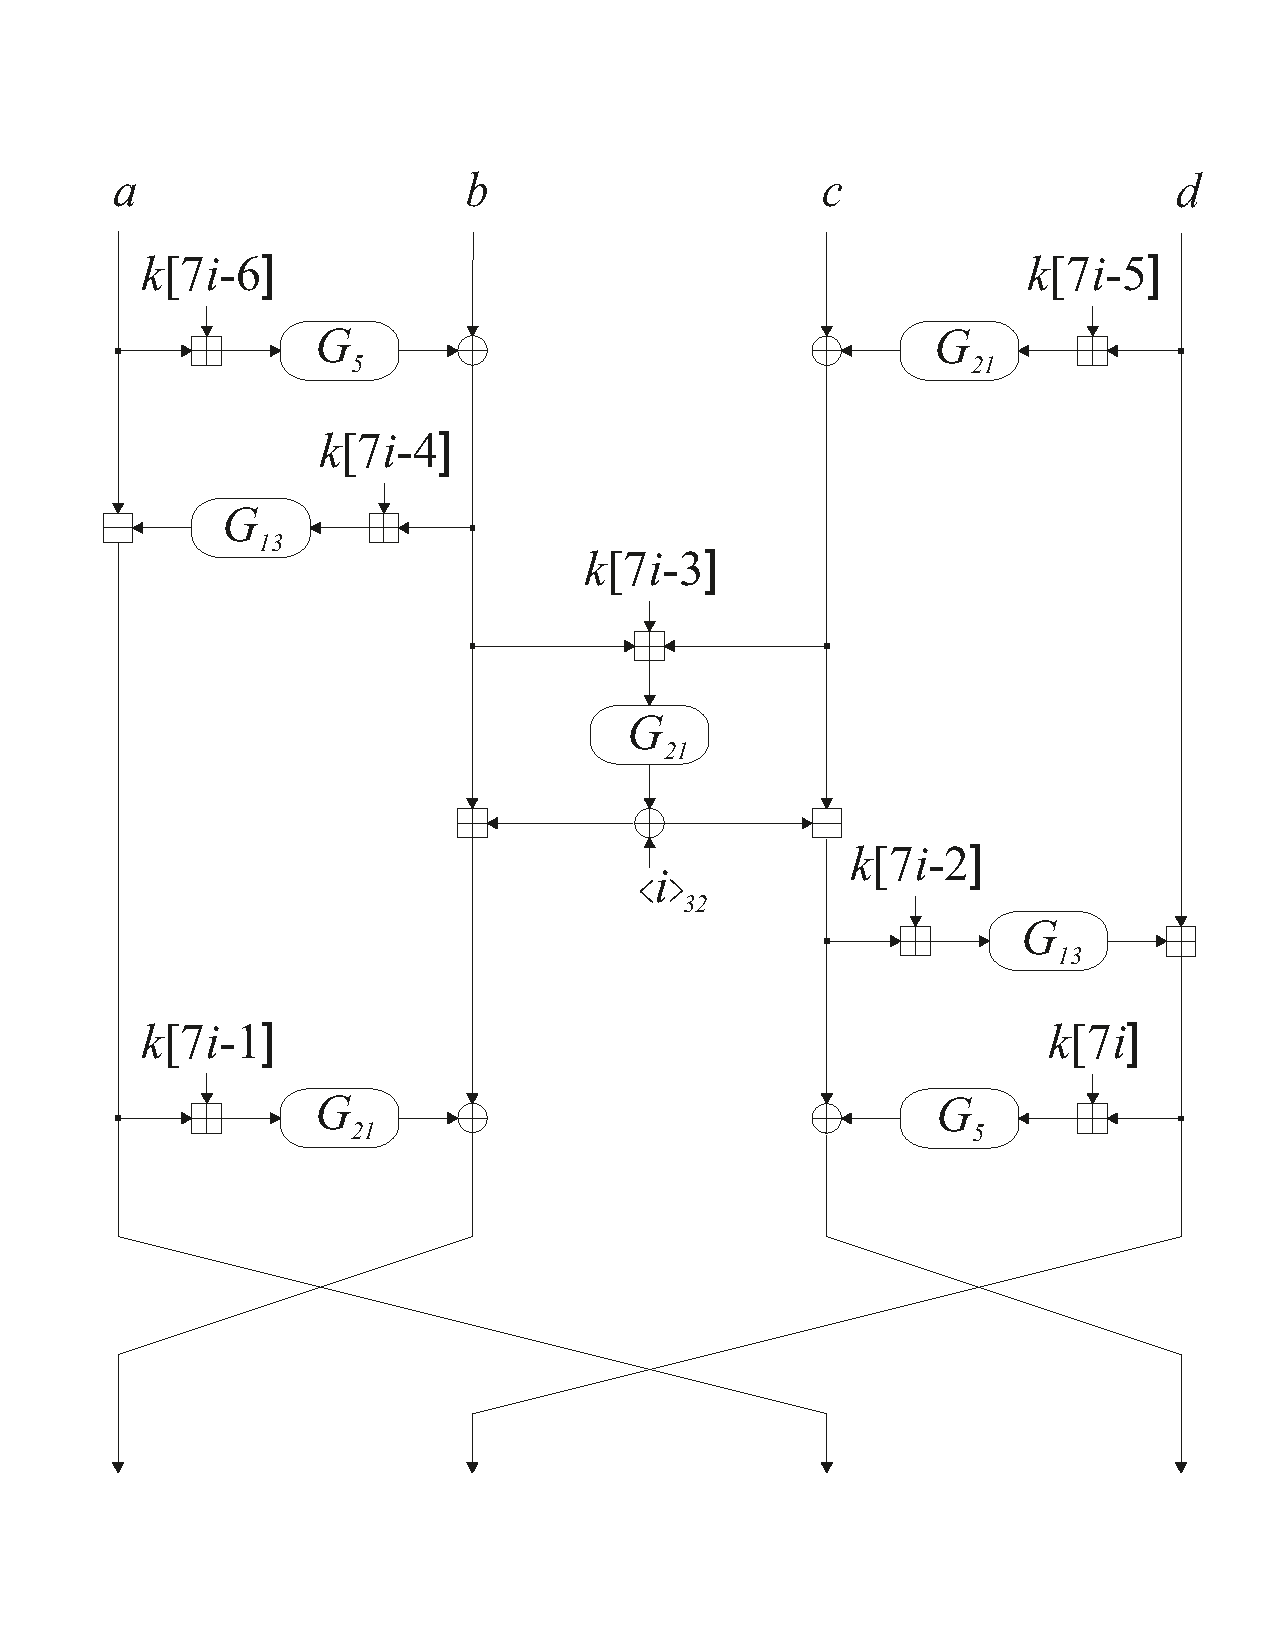
\includegraphics[width=10cm]{../figs/belt-round}
\end{center}
\caption{Вычисления на $i$-м такте зашифрования}\label{Figure.BLOCK.Round}
\end{figure}

\subsection{Алгоритм расшифрования}\label{BLOCK.Decr}

Расшифрование~$\algname{belt-block}^{-1}(Y,K)$ выполняется
следующим образом: 
\begin{enumerate}
\item
Определить $(Y_1,Y_2,Y_3,Y_4)=\Split(Y,32)$.
\item
Определить $(K_1,K_2,\ldots,K_8)=\Split(K,32)$.
\item
Обозначить $k[i]=K_{(i-1)\bmod 8 + 1}$, $i=1,2,\ldots,56$.
\item
Установить $a\leftarrow Y_1$, $b\leftarrow Y_2$, 
$c\leftarrow Y_3$, $d\leftarrow Y_4$.
\item
Для $i=8,7,\ldots,1$ выполнить:
\begin{enumerate}
\item
$b\leftarrow b\oplus G_{5}(a\boxplus k[7i])$;
\item
$c\leftarrow c\oplus G_{21}(d\boxplus k[7i-1])$;
\item
$a\leftarrow a\boxminus G_{13}(b\boxplus k[7i-2])$;
\item
$e\leftarrow G_{21}(b\boxplus c\boxplus k[7i-3])\oplus \itob{i}_{32}$;
\item
$b\leftarrow b\boxplus e$;
\item
$c\leftarrow c\boxminus e$;
\item
$d\leftarrow d\boxplus G_{13}(c\boxplus k[7i-4])$;
\item
$b\leftarrow b\oplus G_{21}(a\boxplus k[7i-5])$;
\item
$c\leftarrow c\oplus G_{5}(d\boxplus k[7i-6])$;
\item
$a\leftrightarrow b$;
\item
$c\leftrightarrow d$;
\item
$a\leftrightarrow d$.
\end{enumerate}
\item
Установить~$X\leftarrow c\parallel a\parallel d\parallel b$.
\item
Возвратить $X$.
\end{enumerate}

\section{Шифрование широкого блока}\label{WBLOCK}

\subsection{Интерфейс}\label{WBLOCK.IFace}

Шифрование широкого блока задается алгоритмами зашифрования~$\algname{belt-wblock}$
и расшифрования~$\algname{belt-wblock}^{-1}$.

Входными данными $\algname{belt-wblock}$ являются слово~$X\in\{0,1\}^{8*}$ 
и ключ~$K\in\{0,1\}^{256}$. Длина~$X$ должна быть не меньше~$256$.
%
Выходными данными является зашифрованное слово~$Y\in\{0,1\}^{|X|}$.

Входными данными $\algname{belt-wblock}^{-1}$ являются зашифрованное слово~$Y\in\{0,1\}^{8*}$ 
и ключ~$K\in\{0,1\}^{256}$. Длина~$Y$ должна быть не меньше~$256$.
%
Выходными данными является расшифрованное слово~$X\in\{0,1\}^{|Y|}$.

Используется алгоритм~$\algname{belt-block}$, определенный в~\ref{BLOCK}.

\subsection{Переменные}\label{WBLOCK.Vars}

Используются переменные~$r\in\{0,1\}^*$ и~$s\in\{0,1\}^{128}$.
Длина~$r$ совпадает с длиной входного слова~$X$ или~$Y$.

\subsection{Алгоритм зашифрования}\label{WBLOCK.Encr}

Зашифрование~$\algname{belt-wblock}(X,K)$ выполняется следующим образом:
\begin{enumerate}
\item
Установить
$r\leftarrow X$.
\item
Представить~$r$ двумя способами:
\begin{enumerate}
\item
в виде набора блоков $(r_1,r_2,\ldots,r_n)=\Split(r,128)$;
\item
в форме $r=r^{**}\parallel r^*$, где $|r^*|=128$.
\end{enumerate}
\item
Для $i=1,2,\ldots,2n$ выполнить:
\begin{enumerate}
\item
$s\leftarrow r_1\oplus r_2\oplus\ldots\oplus r_{n-1}$;

\item
$r^*\leftarrow r^*\oplus \algname{belt-block}(s,K)\oplus
\itob{i}_{128}$;

\item
$r\leftarrow \ShLo^{128}(r)$;

\item
$r^*\leftarrow s$.
\end{enumerate}

\item
Установить
$Y\leftarrow r$.

\item
Возвратить~$Y$.
\end{enumerate}

\subsection{Алгоритм расшифрования}\label{WBLOCK.Decr}

Расшифрование~$\algname{belt-wblock}^{-1}(Y,K)$ выполняется 
следующим образом: 
\begin{enumerate}
\item
Установить $r\leftarrow Y$.
\item
Представить~$r$ двумя способами:
\begin{enumerate}
\item
в виде набора блоков $(r_1,r_2,\ldots,r_n)=\Split(r,128)$;
\item
в форме $r=r^{**}\parallel r^*$, где $|r^*|=128$.
\end{enumerate}
\item
Для $i=2n,\ldots,2,1$ выполнить:
\begin{enumerate}
\item
$s\leftarrow r^*$;
\item
$r\leftarrow \ShHi^{128}(r)$;
\item
$r^*\leftarrow r^*\oplus \algname{belt-block}(s,K)\oplus
\itob{i}_{128}$;
\item
$r_1\leftarrow s\oplus r_2\oplus\ldots\oplus r_{n-1}$.
\end{enumerate}
\item
Установить
$X\leftarrow r$.
\item
Возвратить~$X$.
\end{enumerate}

\section{Cжатие}\label{COMPR}

\subsection{Интерфейс}\label{COMPR.IFace}

Cжатие задается алгоритмом~$\algname{belt-compress}$.

Входными данными $\algname{belt-compress}$ является слово~$X\in\{0,1\}^{512}$.
%
Выходными данными являются слова~$S\in\{0,1\}^{128}$ 
и~$Y\in\{0,1\}^{256}$. 
%
Слово~$S$ является промежуточным результатом сжатия~$X$,
этот выход может игнорироваться.
%
Слово~$Y$ является окончательным результатом сжатия.

Используется алгоритм~$\algname{belt-block}$, определенный в~\ref{BLOCK}.

\subsection{Алгоритм сжатия}\label{COMPR.Alg}

Сжатие~$\algname{belt-compress}(X)$ выполняется следующим образом:
%
\begin{enumerate}
\item
Определить $(X_1,X_2,X_3,X_4)=\Split(X,128)$.
\item
Установить
$S\leftarrow\algname{belt-block}(X_3\oplus X_4,X_1\parallel X_2)\oplus X_3\oplus X_4$.
\item
Установить
$Y_1\leftarrow\algname{belt-block}(X_1,S\parallel X_4)\oplus X_1$.
\item
Установить
$Y_2\leftarrow\algname{belt-block}(X_2,(S\oplus 1^{128})\parallel X_3)\oplus X_2$.
\item
Возвратить~$(S,Y)$, где $Y=Y_1\parallel Y_2$.
\end{enumerate}



\chapter{Алгоритмы шифрования и контроля целостности}\label{CORE}

\section{Шифрование в режиме простой замены}\label{ECB}

\subsection{Интерфейс}\label{ECB.IFace}

Шифрование в режиме простой замены задается алгоритмами 
зашифрования~$\algname{belt-ecb}$ и расшифрования~$\algname{belt-ecb}^{-1}$.

Входными данными $\algname{belt-ecb}$ являются сообщение~$X\in\{0,1\}^*$ и 
ключ~$K\in\{0,1\}^{256}$. 
%
Длина $X$ должна быть не меньше~$128$.
%
Выходными данными является зашифрованное сообщение~$Y\in\{0,1\}^{|X|}$.

Входными данными $\algname{belt-ecb}^{-1}$ являются зашифрованное 
сообщение~$Y\in\{0,1\}^*$ и ключ~$K\in\{0,1\}^{256}$. 
%
Длина $Y$ должна быть не меньше~$128$.
%
Выходными данными является расшифрованное сообщение~$X\in\{0,1\}^{|Y|}$.

Используются алгоритмы~$\algname{belt-block}$ и~$\algname{belt-block}^{-1}$, 
определенные в~\ref{BLOCK}.

\subsection{Переменные}\label{ECB.Vars}

Пусть $m=|X|\bmod 128$ при зашифровании 
и $m=|Y|\bmod 128$ при расшифровании.

Если $m\neq 0$, то используется переменная~$r\in\{0,1\}^{128-m}$.

\subsection{Алгоритм зашифрования}\label{ECB.Encr}

Зашифрование~$\algname{belt-ecb}(X,K)$ выполняется следующим образом: 
\begin{enumerate}
\item
Определить $(X_1,X_2,\ldots,X_n)=\Split(X,128)$.
\item
Если $|X_n|=128$, то:
\begin{enumerate}
\item
для $i=1,2,\ldots,n$ выполнить: $Y_i\leftarrow \algname{belt-block}(X_i,K)$.
\end{enumerate}

\item
Иначе, если $|X_n|<128$, то:
\begin{enumerate}
\item
для $i=1,2,\ldots,n-2$ выполнить: $Y_i\leftarrow \algname{belt-block}(X_i,K)$;

\item
$(Y_n\parallel r)\leftarrow \algname{belt-block}(X_{n-1},K)$;

\item
$Y_{n-1}\leftarrow \algname{belt-block}(X_n\parallel r,K)$.
\end{enumerate}

\item
Возвратить~$Y=Y_1\parallel Y_2\parallel\ldots\parallel Y_n$.
\end{enumerate}

\subsection{Алгоритм расшифрования}\label{ECB.Decr}

Расшифрование~$\algname{belt-ecb}^{-1}(Y,K)$ выполняется следующим образом: 
\begin{enumerate}
\item
Определить $(Y_1,Y_2,\ldots,Y_n)=\Split(Y,128)$.
\item
Если $|Y_n|=128$, то:
\begin{enumerate}
\item
для $i=1,2,\ldots,n$ выполнить: $X_i\leftarrow \algname{belt-block}^{-1}(Y_i,K)$.
\end{enumerate}
\item
Иначе, если $|Y_n|<128$, то:
\begin{enumerate}
\item
для $i=1,2,\ldots,n-2$ 
выполнить: $X_i\leftarrow \algname{belt-block}^{-1}(Y_i,K)$;
\item
$(X_n\parallel r)\leftarrow \algname{belt-block}^{-1}(Y_{n-1},K)$;
\item
$X_{n-1}\leftarrow \algname{belt-block}^{-1}(Y_n\parallel r,K)$.
\end{enumerate}
\item
Возвратить~$X=X_1\parallel X_2\parallel\ldots\parallel X_n$.
\end{enumerate}

\section{Шифрование в режиме сцепления блоков}\label{CBC}

\subsection{Интерфейс}\label{CBC.IFace}

Шифрование в режиме сцепления блоков задается алгоритмами 
зашифрования~$\algname{belt-cbc}$ и расшифрования~$\algname{belt-cbc}^{-1}$.

Входными данными $\algname{belt-cbc}$ являются сообщение~$X\in\{0,1\}^*$, 
ключ~$K\in\{0,1\}^{256}$ и синхропосылка~$S\in\{0,1\}^{128}$. 
%
Длина $X$ должна быть не меньше $128$.
%
Выходными данными является зашифрованное сообщение~$Y\in\{0,1\}^{|X|}$.

Входными данными $\algname{belt-cbc}^{-1}$ являются зашифрованное 
сообщение~$Y\in\{0,1\}^*$, ключ~$K\in\{0,1\}^{256}$ и 
синхропосылка~$S\in\{0,1\}^{128}$.  
%
Длина $Y$ должна быть не меньше $128$.
%
Выходными данными является расшифрованное сообщение~$X\in\{0,1\}^{|Y|}$.

Используются алгоритмы~$\algname{belt-block}$ и~$\algname{belt-block}^{-1}$, 
определенные в~\ref{BLOCK}.

\subsection{Переменные}

Пусть $m=|X|\bmod 128$ при зашифровании 
и $m=|Y|\bmod 128$ при расшифровании.

Если $m\neq 0$, то используется переменная~$r\in\{0,1\}^{128-m}$.

\subsection{Алгоритм зашифрования}

Зашифрование~$\algname{belt-cbc}(X,K,S)$ выполняется следующим образом: 
\begin{enumerate}
\item
Определить $(X_1,X_2,\ldots,X_n)=\Split(X,128)$.
\item
Обозначить~$Y_0=S$.
\item
Если $|X_n|=128$, то
\begin{enumerate}
\item
для $i=1,2,\ldots,n$ выполнить: 
$Y_i\leftarrow \algname{belt-block}(X_i\oplus Y_{i-1},K)$.
\end{enumerate}
\item
Иначе, если $|X_n|<128$, то
\begin{enumerate}
\item
для $i=1,2,\ldots,n-2$ выполнить: 
$Y_i\leftarrow \algname{belt-block}(X_i\oplus Y_{i-1},K)$;
\item
$(Y_n\parallel r)\leftarrow \algname{belt-block}(X_{n-1}\oplus Y_{n-2},K)$;
\item
$Y_{n-1}\leftarrow \algname{belt-block}((X_n\oplus Y_n)\parallel r,K)$.
\end{enumerate}
\item
Возвратить
$Y=Y_1\parallel Y_2\parallel\ldots\parallel Y_n$.
\end{enumerate}

\subsection{Алгоритм расшифрования}

Расшифрование~$\algname{belt-cbc}^{-1}(Y,K,S)$ выполняется следующим образом: 
\begin{enumerate}
\item
Определить $(Y_1,Y_2,\ldots,Y_n)=\Split(Y,128)$.
\item
Обозначить~$Y_0=S$.
\item
Если $|Y_n|=128$, то
\begin{enumerate}
\item
для $i=1,2,\ldots,n$ выполнить: 
$X_i\leftarrow \algname{belt-block}^{-1}(Y_i,K)\oplus Y_{i-1}$.
\end{enumerate}
\item
Иначе, если $|Y_n|<128$, то
\begin{enumerate}
\item
для $i=1,2,\ldots,n-2$ выполнить: 
$X_i\leftarrow \algname{belt-block}^{-1}(Y_i,K)\oplus Y_{i-1}$;
\item
$(X_n\parallel r)\leftarrow \algname{belt-block}^{-1}(Y_{n-1},K)\oplus 
(Y_n\parallel 0^{128-|Y_n|})$;
\item
$X_{n-1}\leftarrow \algname{belt-block}^{-1}(Y_n\parallel r,K)\oplus Y_{n-2}$.
\end{enumerate}
\item
Возвратить
$X=X_1\parallel X_2\parallel\ldots\parallel X_n$.
\end{enumerate}

\section{Шифрование в режиме гаммирования с обратной связью}\label{CFB}

\subsection{Интерфейс}\label{CFB.IFace}

Шифрование в режиме гаммирования с обратной связью задается алгоритмами 
зашифрования~$\algname{belt-cfb}$ и расшифрования~$\algname{belt-cfb}^{-1}$.

Входными данными $\algname{belt-cfb}$ являются сообщение~$X\in\{0,1\}^*$, 
ключ~$K\in\{0,1\}^{256}$ и синхропосылка~$S\in\{0,1\}^{128}$.
%
Выходными данными является зашифрованное сообщение~$Y\in\{0,1\}^{|X|}$.

Входными данными $\algname{belt-cfb}^{-1}$ являются зашифрованное 
сообщение~$Y\in\{0,1\}^*$, ключ~$K\in\{0,1\}^{256}$ и 
синхропосылка~$S\in\{0,1\}^{128}$. 
%
Выходными данными является расшифрованное сообщение~$X\in\{0,1\}^{|Y|}$.

Используется алгоритм~$\algname{belt-block}$, определенный в~\ref{BLOCK}.

\subsection{Алгоритм зашифрования}\label{CFB.Encr}

Зашифрование~$\algname{belt-cfb}(X,K,S)$ выполняется следующим образом: 
\begin{enumerate}
\item
Определить~$(X_1,X_2,\ldots,X_n)=\Split(X, 128)$.
\item
Обозначить~$Y_0=S$.
\item
Для $i=1,2,\ldots,n$ выполнить:
$Y_i\leftarrow X_i\oplus\Lo(\algname{belt-block}(Y_{i-1},K), |X_i|)$.
\item
Возвратить
$Y=Y_1\parallel Y_2\parallel\ldots\parallel Y_n$.
\end{enumerate}

\subsection{Алгоритм расшифрования}\label{CFB.Decr}

Расшифрование~$\algname{belt-cfb}^{-1}(Y,K,S)$ выполняется следующим образом: 
\begin{enumerate}
\item
Определить~$(Y_1,Y_2,\ldots,Y_n)=\Split(Y, 128)$.
\item
Обозначить~$Y_0=S$.
\item
Для $i=1,2,\ldots,n$ выполнить: 
$X_i\leftarrow X_i\oplus\Lo(\algname{belt-block}(Y_{i-1},K), |Y_i|)$.
\item
Возвратить
$X=X_1\parallel X_2\parallel\ldots\parallel X_n$.
\end{enumerate}

\section{Шифрование в режиме счетчика}\label{CTR}

\subsection{Интерфейс}\label{CTR.IFace}

Шифрование в режиме счетчика задается алгоритмами 
зашифрования~$\algname{belt-ctr}$ и расшифрования~$\algname{belt-ctr}^{-1}$.

Входными данными $\algname{belt-ctr}$ являются сообщение~$X\in\{0,1\}^*$, 
ключ~$K\in\{0,1\}^{256}$ и синхропосылка~$S\in\{0,1\}^{128}$.
%
Выходными данными является зашифрованное сообщение~$Y\in\{0,1\}^{|X|}$.

Входными данными $\algname{belt-ctr}^{-1}$ являются зашифрованное 
сообщение~$Y\in\{0,1\}^*$, ключ~$K\in\{0,1\}^{256}$ и 
синхропосылка~$S\in\{0,1\}^{128}$. 
%
Выходными данными является расшифрованное сообщение~$X\in\{0,1\}^{|Y|}$.

Используется алгоритм~$\algname{belt-block}$, определенный в~\ref{BLOCK}.

\subsection{Переменные}\label{CTR.Vars}

Используется переменная~$s\in\{0,1\}^{128}$.

\subsection{Алгоритм зашифрования}\label{CTR.Encr}

Зашифрование~$\algname{belt-ctr}(X,K,S)$ выполняется следующим образом:
\begin{enumerate}
\item
Определить $(X_1,X_2,\ldots,X_n)=\Splitz(X,128)$.
\item
Установить 
$s\leftarrow \algname{belt-block}(S,K)$.
\item
Для $i=1,2,\ldots,n$ выполнить:
\begin{enumerate}
\item
$s\leftarrow s\boxplus\itob{1}_{128}$,
\item
$Y_i\leftarrow X_i\oplus\Lo(\algname{belt-block}(s,K),|X_i|)$.
\end{enumerate}
\item
Возвратить~$Y=Y_1\parallel Y_2\parallel\ldots\parallel Y_n$.
\end{enumerate}

\subsection{Алгоритм расшифрования}\label{CTR.Decr}

Расшифрование~$\algname{belt-ctr}^{-1}(Y,K,S)$ выполняется следующим образом:
\begin{enumerate}
\item
Определить $(Y_1,Y_2,\ldots,Y_n)=\Splitz(Y,128)$.
\item
Установить 
$s\leftarrow \algname{belt-block}(S,K)$.
\item
Для $i=1,2,\ldots,n$ выполнить:
\begin{enumerate}
\item
$s\leftarrow s\boxplus\itob{1}_{128}$,
\item
$X_i\leftarrow Y_i\oplus\Lo(\algname{belt-block}(s,K),|Y_i|)$.
\end{enumerate}
\item
Возвратить~$X=X_1\parallel X_2\parallel\ldots\parallel X_n$.
\end{enumerate}

\section{Выработка имитовставки}\label{MAC}

\subsection{Интерфейс}\label{MAC.IFace}

Выработка имитовставки задается алгоритмом~$\algname{belt-mac}$.

Входными данными~$\algname{belt-mac}$ являются
сообщение~$X\in\{0,1\}^*$ и ключ~$K\in\{0,1\}^{256}$.
%
Выходными данными является имитовставка~$T\in\{0,1\}^{64}$.

Используется алгоритм~$\algname{belt-block}$, 
определенный в~\ref{BLOCK}.

\subsection{Вспомогательные преобразования и переменные}\label{MAC.Aux}

\paragraph{Преобразования $\varphi_1$ и $\varphi_2$.}
Преобразования $\varphi_1,\varphi_2\colon\{0,1\}^{128}\to\{0,1\}^{128}$
действуют на слово 
$u=u_1\parallel u_2\parallel u_3\parallel u_4$, 
$u_i\in\{0,1\}^{32}$, по правилам:
\begin{align*}
\varphi_1(u)&=u_2\parallel u_3\parallel u_4\parallel(u_1\oplus u_2),\\
\varphi_2(u)&=(u_1\oplus u_4)\parallel u_1\parallel u_2\parallel u_3.
\end{align*}

\paragraph{Отображение~$\psi$.}
Отображение $\psi$ ставит в соответствие двоичному слову $u$,
длина которого меньше $128$, слово
$
\psi(u)=u\parallel 1\parallel 0^{127-|u|}
$
длины~$128$.

\paragraph{Переменные.}
Используются переменные~$r,s\in\{0,1\}^{128}$.

\subsection{Алгоритм выработки имитовставки}\label{MAC.Alg}

Выработка имитовставки $\algname{belt-mac}(X,K)$ выполняется следующим образом:
\begin{enumerate}
\item
Определить $(X_1,X_2,\ldots,X_n)=\Splita(X,128)$.
\item
Установить
$s\leftarrow 0^{128}$, $r\leftarrow \algname{belt-block}(s,K)$.
\item
Для $i=1,2,\ldots,n-1$ выполнить:
$s\leftarrow \algname{belt-block}(s\oplus X_i,K)$.
\item
Если $|X_n|=128$, то 
$s\leftarrow s\oplus X_n\oplus \varphi_1(r)$.
\item
Иначе, если $|X_n|<128$, то
$s\leftarrow s\oplus\psi(X_n)\oplus\varphi_2(r)$.
\item
Установить
$T\leftarrow\Lo(\algname{belt-block}(s,K), 64)$.
\item
Возвратить~$T$.
\end{enumerate}

\vskip9pt
\begin{note}
Примечание~--- Если $X=\perp$, то $n=1$ и $X_1=\perp$.
\end{note}

\section{Аутентифицированное шифрование данных}\label{AE}

\subsection{Интерфейс}\label{AE.IFace}

Аутентифицированное шифрование данных задается алгоритмами установки 
и снятия защиты. Первая схема аутентифицированного шифрования
представлена алгоритмами $\algname{belt-dwp}$ и~$\algname{belt-dwp}^{-1}$,
вторая~--- алгоритмами $\algname{belt-che}$ и~$\algname{belt-che}^{-1}$. 

Входными данными алгоритма установки защиты ($\algname{belt-dwp}$ или
$\algname{belt-che}$) являются сообщение~$X\in\{0,1\}^*$, ассоциированные
данные~$I\in\{0,1\}^*$, ключ~$K\in\{0,1\}^{256}$ и 
синхропосылка~$S\in\{0,1\}^{128}$. Длины~$X$ и~$I$ должны быть меньше~$2^{64}$. 
%
Выходными данными являются зашифрованное сообщение~$Y\in\{0,1\}^{|X|}$
и имитовставка~$T\in\{0,1\}^{64}$.

Входными данными алгоритма снятия защиты ($\algname{belt-dwp}^{-1}$ или
$\algname{belt-che}^{-1}$) являются зашифрованное
сообщение~$Y\in\{0,1\}^*$, ассоциированные данные~$I\in\{0,1\}^*$,
имитовставка~$T\in\{0,1\}^{64}$, ключ~$K\in\{0,1\}^{256}$ и синхропосылка
$S\in\{0,1\}^{128}$.
%
Длины $Y$ и $I$ должны быть меньше $2^{64}$.
%
Выходными данными является либо признак ошибки~$\perp$, либо расшифрованное 
сообщение~$X\in\{0,1\}^{|Y|}$. 
%
Возврат~$\perp$ означает нарушение целостности входных данных.

Используется алгоритм~$\algname{belt-block}$, 
определенный в~\ref{BLOCK}.

\subsection{Переменные и константы}\label{AE.Vars}

Используются переменные~$s,t\in\{0,1\}^{128}$.

В алгоритмах схемы~1 дополнительно используется переменная~$r\in\{0,1\}^{128}$. 

В алгоритмах схемы~2 используется слово~$C=\hex{02}\parallel 0^{120}$.
Слово представляет многочлен~$C(x)=x$ (см.~\ref{DEFS.Poly}).

\subsection{Алгоритм установки защиты (схема 1)}\label{AE.DWP.Wrap}

Установка защиты~$\algname{belt-dwp}(X,I,K,S)$ выполняется следующим образом:
\begin{enumerate}
\item
Определить 
\begin{enumerate}
\item
$(X_1,X_2,\ldots,X_n)=\Split(X, 128)$;
\item
$(I_1,I_2,\ldots,I_m)=\Split(I, 128)$. 
\end{enumerate}
\item
Установить
\begin{enumerate}
\item
$s\leftarrow\algname{belt-block}(S,K)$;
\item
$r\leftarrow \algname{belt-block}(s,K)$;
\item
$t\leftarrow\hex{B194BAC80A08F53B366D008E584A5DE4}$
(см. строку 1 таблицы~\ref{Table.SBOX}).
\end{enumerate}

\item
Для $i=1,2,\ldots,m$ выполнить:
\begin{enumerate}
\item
$t\leftarrow t\oplus (I_i\parallel 0^{128-|I_i|})$;
\item
$t\leftarrow t\ast r$.
\end{enumerate}

\item
Для $i=1,2,\ldots,n$ выполнить:
\begin{enumerate}
\item
$s\leftarrow s\boxplus\itob{1}_{128}$;
\item
$Y_i\leftarrow X_i\oplus\Lo(\algname{belt-block}(s,K), |X_i|)$;
\item
$t\leftarrow t\oplus (Y_i\parallel 0^{128-|Y_i|})$;
\item
$t\leftarrow t\ast r$.
\end{enumerate}

\item
Установить
$t\leftarrow t\oplus 
(\itob{|I|}_{64}\parallel\itob{|X|}_{64})$.
\item
Установить
$t\leftarrow \algname{belt-block}(t\ast r,K)$.
\item
Установить
$T\leftarrow \Lo(t, 64)$.
\item
Возвратить~$(Y,T)$, 
где~$Y=Y_1\parallel Y_2\parallel\ldots\parallel Y_n$.
\end{enumerate}

\subsection{Алгоритм снятия защиты (схема 1)}\label{AE.DWP.Unwrap}

Снятие защиты~$\algname{belt-dwp}^{-1}(Y,I,T,K,S)$ выполняется следующим образом:
\begin{enumerate}
\item
Определить 
\begin{enumerate}
\item
$(Y_1,Y_2,\ldots,Y_n)=\Split(Y, 128)$;
\item
$(I_1,I_2,\ldots,I_m)=\Split(I, 128)$. 
\end{enumerate}
\item
Установить
\begin{enumerate}
\item
$s\leftarrow\algname{belt-block}(S,K)$;
\item
$r\leftarrow \algname{belt-block}(s,K)$;
\item
$t\leftarrow\hex{B194BAC80A08F53B366D008E584A5DE4}$.
\end{enumerate}

\item
Для $i=1,2,\ldots,m$ выполнить:
\begin{enumerate}
\item
$t\leftarrow t\oplus (I_i\parallel 0^{128-|I_i|})$;
\item
$t\leftarrow t\ast r$.
\end{enumerate}

\item\label{Step.AE.DWP.StepA}
Для $i=1,2,\ldots,n$ выполнить:
\begin{enumerate}
\item
$t\leftarrow t\oplus (Y_i\parallel 0^{128-|Y_i|})$;
\item
$t\leftarrow t\ast r$.
\end{enumerate}

\item
Установить
$t\leftarrow t\oplus 
(\itob{|I|}_{64}\parallel\itob{|Y|}_{64})$.

\item
Установить
$t\leftarrow \algname{belt-block}(t\ast r,K)$.

\item\label{Step.AE.DWP.VerifyMAC}
Если $T\neq \Lo(t, 64)$, то возвратить~$\perp$.

\item\label{Step.AE.DWP.StepD}
Для $i=1,2,\ldots,n$ выполнить:
\begin{enumerate}
\item
$s\leftarrow s\boxplus\itob{1}_{128}$;
\item
$X_i\leftarrow Y_i\oplus \Lo(\algname{belt-block}(s,K),|Y_i|)$.
\end{enumerate}

\item
Возвратить~$X=X_1\parallel X_2\parallel\ldots\parallel X_n$.
\end{enumerate}

\subsection{Алгоритм установки защиты (схема 2)}\label{AE.CHE.Wrap}

Установка защиты~$\algname{belt-che}(X,I,K,S)$ выполняется следующим образом:
\begin{enumerate}
\item
Определить 
\begin{enumerate}
\item
$(X_1,X_2,\ldots,X_n)=\Split(X, 128)$;
\item
$(I_1,I_2,\ldots,I_m)=\Split(I, 128)$. 
\end{enumerate}
\item
Установить
\begin{enumerate}
\item
$s\leftarrow\algname{belt-block}(S,K)$;
\item
$r\leftarrow s$;
\item
$t\leftarrow\hex{B194BAC80A08F53B366D008E584A5DE4}$.
\end{enumerate}

\item
Для $i=1,2,\ldots,m$ выполнить:
\begin{enumerate}
\item
$t\leftarrow t\oplus (I_i\parallel 0^{128-|I_i|})$;
\item
$t\leftarrow t\ast r$.
\end{enumerate}

\item
Для $i=1,2,\ldots,n$ выполнить:
\begin{enumerate}
\item
$s\leftarrow (s\ast C)\oplus\itob{1}_{128}$;
\item
$Y_i\leftarrow X_i\oplus\Lo(\algname{belt-block}(s,K), |X_i|)$;
\item
$t\leftarrow t\oplus (Y_i\parallel 0^{128-|Y_i|})$;
\item
$t\leftarrow t\ast r$.
\end{enumerate}

\item
Установить
$t\leftarrow t\oplus 
(\itob{|I|}_{64}\parallel\itob{|X|}_{64})$.
\item
Установить
$t\leftarrow \algname{belt-block}(t\ast r,K)$.
\item
Установить
$T\leftarrow \Lo(t, 64)$.
\item
Возвратить~$(Y,T)$, 
где~$Y=Y_1\parallel Y_2\parallel\ldots\parallel Y_n$.
\end{enumerate}

\subsection{Алгоритм снятия защиты (схема 2)}\label{AE.CHE.Unwrap}

Снятие защиты~$\algname{belt-che}^{-1}(Y,I,T,K,S)$ выполняется следующим образом:
\begin{enumerate}
\item
Определить 
\begin{enumerate}
\item
$(Y_1,Y_2,\ldots,Y_n)=\Split(Y, 128)$;
\item
$(I_1,I_2,\ldots,I_m)=\Split(I, 128)$. 
\end{enumerate}
\item
Установить
\begin{enumerate}
\item
$s\leftarrow\algname{belt-block}(S,K)$;
\item
$r\leftarrow s$;
\item
$t\leftarrow\hex{B194BAC80A08F53B366D008E584A5DE4}$.
\end{enumerate}

\item
Для $i=1,2,\ldots,m$ выполнить:
\begin{enumerate}
\item
$t\leftarrow t\oplus (I_i\parallel 0^{128-|I_i|})$;
\item
$t\leftarrow t\ast r$.
\end{enumerate}

\item\label{Step.AE.CHE.StepA}
Для $i=1,2,\ldots,n$ выполнить:
\begin{enumerate}
\item
$t\leftarrow t\oplus (Y_i\parallel 0^{128-|Y_i|})$;
\item
$t\leftarrow t\ast r$.
\end{enumerate}

\item
Установить
$t\leftarrow t\oplus (\itob{|I|}_{64}\parallel\itob{|Y|}_{64})$.

\item
Установить
$t\leftarrow\algname{belt-block}(t\ast r,K)$.

\item\label{Step.AE.CHE.VerifyMAC}
Если $T\neq\Lo(t, 64)$, то возвратить~$\perp$.

\item\label{Step.AE.CHE.StepD}
Для $i=1,2,\ldots,n$ выполнить:
\begin{enumerate}
\item
$s\leftarrow (s\ast C)\oplus\itob{1}_{128}$;
\item
$X_i\leftarrow Y_i\oplus \Lo(\algname{belt-block}(s,K), |Y_i|)$.
\end{enumerate}
\item
Возвратить~$X=X_1\parallel X_2\parallel\ldots\parallel X_n$.
\end{enumerate}

\vskip6pt

\begin{note}
Примечание~1~--- Если длина имитовставки, вычисляемой при установке защиты, 
сокращается до~$n$ битов (см.~\ref{COMMON.MAC}), то на вход алгоритма снятия 
защиты должна подаваться сокращенная имитовставка, а проверка~$T\neq\Lo(t,64)$ 
на шаге~\ref{Step.AE.DWP.VerifyMAC} этого алгоритма должна быть изменена на 
проверку~$T\neq\Lo(t,n)$.
\end{note}

\vskip6pt

\begin{note}
Примечание~2~--- В алгоритме снятия защиты расшифрование на 
шаге~\ref{Step.AE.DWP.StepD} может выполняться одновременно 
с вычислением имитовставки на шаге~\ref{Step.AE.DWP.StepA}. 
Однако расшифрование может оказаться бесполезным, если на 
шаге~\ref{Step.AE.DWP.VerifyMAC} имитовставка окажется некорректной.
\end{note}
\section{Аутентифицированное шифрование ключа}\label{KWP}

\subsection{Интерфейс}\label{KWP.IFace}

Аутентифицированное шифрование ключа задается алгоритмами установки 
защиты~$\algname{belt-kwp}$ и снятия защиты~$\algname{belt-kwp}^{-1}$.

Входными данными $\algname{belt-kwp}$ являются защищаемый 
ключ~$X\in\{0,1\}^{8*}$, его заголовок~$I\in\{0,1\}^{128}$ и ключ 
защиты~$K\in\{0,1\}^{256}$. Длина~$X$ должна быть не меньше~$128$.
%
Выходными данными является защищенный ключ~$Y\in\{0,1\}^{|X|+128}$.

Входными данными $\algname{belt-kwp}^{-1}$ являются защищенный
ключ~$Y\in\{0,1\}^*$, его заголовок~$I\in\{0,1\}^{128}$ и ключ
защиты~$K\in\{0,1\}^{256}$.
%
Выходными данными является либо признак ошибки~$\perp$,
либо исходный ключ~$X\in\{0,1\}^{|Y|-128}$.
%
Возврат~$\perp$ означает нарушение целостности входных данных.

Используются алгоритмы~$\algname{belt-wblock}$, $\algname{belt-wblock}^{-1}$
определенные в~\ref{WBLOCK}.

\subsection{Переменные}\label{KWP.Vars}

При снятии защиты используется переменная~$r\in\{0,1\}^{128}$.

\subsection{Алгоритм установки защиты}\label{KWP.Wrap}

Установка защиты~$\algname{belt-kwp}(X,I,K)$ выполняется следующим образом:
\begin{enumerate}
\item
$Y\leftarrow\algname{belt-wblock}(X\parallel I,K)$.

\item
Возвратить~$Y$.
\end{enumerate}

\subsection{Алгоритм снятия защиты}\label{KWP.Unwrap}

Снятие защиты~$\algname{belt-kwp}^{-1}(Y,I,K)$ выполняется следующим образом:
\begin{enumerate}
\item
Если длина~$Y$ не кратна~$8$ или~$|Y|<256$, то возвратить~$\perp$.
\item
$(X\parallel r)\leftarrow \algname{belt-wblock}^{-1}(Y,K)$.
\item
Если $r\neq I$, то возвратить~$\perp$.
\item
Возвратить~$X$.
\end{enumerate}

\section{Хэширование}\label{HASH}

\subsection{Интерфейс}\label{HASH.IFace}

Хэширование задается алгоритмом~$\algname{belt-hash}$.

Входными данными~$\algname{belt-hash}$ является сообщение~$X\in\{0,1\}^*$.
%
Выходными данными является хэш-значение~$Y\in\{0,1\}^{256}$.

Используется алгоритм~$\algname{belt-compress}$, определенный в~\ref{COMPR}.

\subsection{Переменные}\label{HASH.Vars}

Используются переменные~$r,s,t\in\{0,1\}^{128}$ и~$h\in\{0,1\}^{256}$.

\subsection{Алгоритм хэширования}\label{HASH.Alg}

Хэширование~$\algname{belt-hash}(X)$ выполняется следующим образом:
\begin{enumerate}
\item
Определить $(X_1,X_2,\ldots,X_n)=\Split(X, 256)$.

\item
Установить
\begin{enumerate}
\item
$r\leftarrow \itob{|X|}_{128}$;
\item
$s\leftarrow 0^{128}$;
\item
$h\leftarrow\hex{B194BAC80A08F53B366D008E584A5DE48504FA9D1BB6C7AC252E72C202FDCE0D}$ 
(см. первые две строки таблицы~\ref{Table.SBOX});
\item
$X_n\leftarrow X_n \parallel 0^{256-|X_n|}$.
\end{enumerate}

\item
Для $i=1,2,\ldots,n$ выполнить:
\begin{enumerate}
\item
$(t,h)\leftarrow\algname{belt-compress}(X_i\parallel h)$;
\item
$s\leftarrow s\oplus t$.
\end{enumerate}

\item
Установить 
$(\perp,Y)\leftarrow\algname{belt-compress}(r\parallel s\parallel h)$.

\item
Возвратить $Y$.
\end{enumerate}

\vskip9pt
\begin{note}
Примечание~--- Если $X=\perp$, то $n=1$ и $X_1=\perp$.
\end{note}

\section{Дисковое шифрование}\label{DSK}

\subsection{Интерфейс}\label{DSK.IFace}

Блоковое дисковое шифрование задается алгоритмами 
зашифрования~$\algname{belt-bde}$ и расшифрования~$\algname{belt-bde}^{-1}$.
%
Секторное дисковое шифрование задается алгоритмами 
зашифрования~$\algname{belt-sde}$ и расшифрования~$\algname{belt-sde}^{-1}$.

Входными данными~$\algname{belt-bde}$, $\algname{belt-sde}$ являются 
сообщение~$X\in\{0,1\}^{128*}$, ключ~$K\in\{0,1\}^{256}$ и 
синхропосылка~$S\in\{0,1\}^{128}$. 
%
При блоковом шифровании длина~$X$ должна быть не меньше~$128$, при 
секторном~--- не меньше~$256$.
%
Выходными данными является зашифрованное сообщение~$Y\in\{0,1\}^{|X|}$.

Входными данными~$\algname{belt-bde}^{-1}$, $\algname{belt-sde}^{-1}$ являются 
зашифрованное сообщение~$Y\in\{0,1\}^{128*}$, ключ~$K\in\{0,1\}^{256}$ и 
синхропосылка~$S\in\{0,1\}^{128}$. 
%
При блоковом шифровании длина~$Y$ должна быть не меньше~$128$, при 
секторном~--- не меньше~$256$.
%
Выходными данными является расшифрованное сообщение~$X\in\{0,1\}^{|Y|}$.

Слова~$X$ и~$Y$ представляют собой содержимое дискового сектора до и после
зашифрования. Синхропосылка~$S$ строится по номеру сектора.
Например, $S=\itob{D}_{128}$ для сектора номер $D$.

Используются алгоритмы~$\algname{belt-block}$ и~$\algname{belt-block}^{-1}$, 
определенные в~\ref{BLOCK}. 
%
При секторном шифровании дополнительно используются 
алгоритмы~$\algname{belt-wblock}$ и~$\algname{belt-wblock}^{-1}$, 
определенные в~\ref{WBLOCK}.  

\subsection{Переменные и константы}\label{DSK.Vars}

Используется переменная~$s\in\{0,1\}^{128}$. 

В алгоритмах~$\algname{belt-bde}$, $\algname{belt-bde}^{-1}$ 
используется слово~$C=\hex{02}\parallel 0^{120}$.
Слово представляет многочлен~$C(x)=x$ (см.~\ref{DEFS.Poly}).

\subsection{Алгоритм блокового зашифрования}\label{DSK.BDE.Encr}

Зашифрование~$\algname{belt-bde}(X,K,S)$ выполняется следующим образом: 
\begin{enumerate}
\item
Определить~$(X_1,X_2,\ldots,X_n)=\Split(X, 128)$.
\item
Установить~$s\leftarrow \algname{belt-block}(S,K)$.
\item
Для~$i=1,2,\ldots,n$ выполнить: 
\begin{enumerate}
\item
$s\leftarrow s \ast C$;
\item
$Y_i\leftarrow\algname{belt-block}(X_i\oplus s, K)\oplus s$.
\end{enumerate}
\item
Возвратить~$Y=Y_1\parallel Y_2\parallel\ldots\parallel Y_n$.
\end{enumerate}

\subsection{Алгоритм блокового расшифрования}\label{DSK.BDE.Decr}

Расшифрование~$\algname{belt-bde}^{-1}(Y,K,S)$ выполняется следующим образом: 
\begin{enumerate}
\item
Определить~$(Y_1,Y_2,\ldots,Y_n)=\Split(Y,128)$.
\item
Установить~$s\leftarrow\algname{belt-block}(S,K)$.
\item
Для~$i=1,2,\ldots,n$ выполнить: 
\begin{enumerate}
\item
$s\leftarrow s \ast C$;
\item
$X_i\leftarrow\algname{belt-block}^{-1}(Y_i\oplus s, K)\oplus s$.
\end{enumerate}
\item
Возвратить~$X=X_1\parallel X_2\parallel\ldots\parallel X_n$.
\end{enumerate}

\subsection{Алгоритм секторного зашифрования}\label{DSK.SDE.Encr}

Зашифрование~$\algname{belt-sde}(X,K,S)$ выполняется следующим образом: 
\begin{enumerate}
\item
Установить~$Y\leftarrow X$.
\item
Записать~$Y=Y_1\parallel Y_2$, где $|Y_1|=128$.
\item
Установить~$s\leftarrow \algname{belt-block}(S,K)$.
\item
Установить~$Y_1\leftarrow Y_1\oplus s$.
\item
Установить~$Y\leftarrow\algname{belt-wblock}(Y,K)$.
\item
Установить~$Y_1\leftarrow Y_1\oplus s$.
\item
Возвратить~$Y$.
\end{enumerate}

\subsection{Алгоритм секторного расшифрования}\label{DSK.SDE.Decr}

Расшифрование~$\algname{belt-sde}^{-1}(Y,K,S)$ выполняется следующим образом: 
\begin{enumerate}
\item
Установить~$X\leftarrow Y$.
\item
Записать~$X=X_1\parallel X_2$, где $|X_1|=128$.
\item
Установить~$s\leftarrow \algname{belt-block}(S,K)$.
\item
Установить~$X_1\leftarrow X_1\oplus s$.
\item
Установить~$X\leftarrow\algname{belt-wblock}^{-1}(X,K)$.
\item
Установить~$X_1\leftarrow X_1\oplus s$.
\item
Возвратить~$X$.
\end{enumerate}

\section{Шифрование с сохранением формата}\label{FMT}

\subsection{Интерфейс}\label{FMT.IFace}

Шифрование с сохранением формата задается алгоритмами зашифрования
$\algname{belt-fmt}$ и расшифрования~$\algname{belt-fmt}^{-1}$.

Входными данными $\algname{belt-fmt}$ являются 
слово~$X\in\ZZ_m^n$, ключ~$K\in\{0,1\}^{256}$ 
и синхропосылка~$S\in\{0,1\}^{128}$.
%
Выходными данными является зашифрованное слово~$Y\in\ZZ_m^n$.

Входными данными $\algname{belt-fmt}^{-1}$ являются 
зашифрованное слово~$Y\in\ZZ_m^n$, ключ~$K\in\{0,1\}^{256}$ 
и синхропосылка~$S\in\{0,1\}^{128}$.
%
Выходными данными является расшифрованное слово~$X\in\ZZ_m^n$.

Размер алфавита~$\ZZ_m$ и длина~$n$ входного и выходного слов 
должны принадлежать интервалу~$\{2,3,\ldots,65536\}$.

Используются алгоритмы~$\algname{belt-block}$ и~$\algname{belt-wblock}$,
определенные в~\ref{BLOCK} и~\ref{WBLOCK}.

\subsection{Подготовка входных данных}\label{FMT.Data}

Длина~$n$ записывается в виде суммы~$n_1+n_2$,
где~$n_1=\lceil n/2\rceil$, $n_2=\lfloor n/2\rfloor$.
%
По слагаемому~$n_i$, $i=1,2$, определяется минимальное натуральное~$b_i$ 
такое, что:
\begin{enumerate}
\item[1)]
$b_i$ кратно~$64$;
\item[2)]
$2^{b_i}\geq m^{n_i}$.
\end{enumerate}

Синхропосылка~$S$ разбивается на фрагменты~$(S_1,S_2,S_3,S_4)=\Split(S,32)$. 
%
Дополнительно строятся слова~$S_0$ и~$S_5$, описывающие формат: 
$S_0=S_5=\itob{m}_{16}\parallel\itob{n}_{16}$. 

\subsection{Вспомогательные алгоритмы, переменные и обозначения}\label{FMT.Aux}

{\bf Алгоритм~\algname{belt-32block}}.
Используется алгоритм~\algname{belt-32block},
который принимает на вход слово~$t\in\{0,1\}^{192}$ и ключ~$K\in\{0,1\}^{256}$
и возвращает преобразованное слово~$t$. В слове~$t$ выделяются 
фрагменты $(t_1,t_2,t_3)=\Split(t,64)$.

Шаги алгоритма:
\begin{enumerate}
\item
Для $i=1,2,3$:
\begin{enumerate}
\item
$(t_2\parallel t_3)\leftarrow
\algname{belt-block}(t_2\parallel t_3,K)\oplus \itob{i}_{64}$; 
\item
$t\leftarrow t_2\parallel t_3\parallel(t_1\oplus t_2)$.
\end{enumerate}
\item
Возвратить~$t$.
\end{enumerate}

{\bf Переменная~$r$}.
Используется переменная~$r\in\ZZ_m^n$.
Переменная записывается в виде~$r=r_1\parallel r_2$,
$|r_i|=n_i$.

{\bf Переменные~$t_1$, $t_2$}.
Используются переменные~$t_1\in\{0,1\}^{64+b_1}$ 
и~$t_2\in\{0,1\}^{64+b_2}$.

{\bf Обозначение~\algname{str2bin}}.
Для~$j\in\{1,2\}$ и~$u\in\ZZ_m^*$ через~$\algname{str2bin}(u,b_j)$ 
обозначается двоичное слово~$\itob{\btoi{u}_m}_{b_j}$.

{\bf Обозначение~\algname{bin2str}}.
Для~$j\in\{1,2\}$ и~$t\in\{0,1\}^{64*}$ через~$\algname{bin2str}(t,n_j)$ 
обозначается слово~$\itob{\btoi{t}}_{m,n_j}$. 

{\bf Обозначение~\algname{roundf}}.
Пусть $t\in\{0,1\}^{64*}$, причем~$|t|\geq 128$.
Обозначение~$\algname{roundf}(t,K)$ раскрывается как:
\begin{enumerate}
\item[1)]
$\algname{belt-block}(t,K)$ при $|t|=128$;
\item[2)]
$\algname{belt-32block}(t,K)$ при $|t|=192$ и
\item[3)]
$\algname{belt-wblock}(t,K)$ при $|t|\geq 256$.
\end{enumerate}

\subsection{Константы}\label{FMT.Const}

В алгоритмах используются константы $C_0,C_1,\ldots,C_5\in\{0,1\}^{32}$.
Константы определяются по~первым двум строкам таблицы~\ref{Table.SBOX}
и имеют следующий вид:
\begin{align*}
&
C_0 = \hex{B194BAC8},\quad
C_1 = \hex{0A08F53B},\quad
C_2 = \hex{366D008E},\quad
C_3 = \hex{584A5DE4},\\
&
C_4 = \hex{8504FA9D},\quad
C_5 = \hex{1BB6C7AC}.
\end{align*}

\subsection{Алгоритм зашифрования}

Зашифрование~$\algname{belt-fmt}(X,K,S)$ выполняется следующим образом:
\begin{enumerate}
\item
Установить $r\leftarrow X$.
\item
Для $i=1,2,3$:
\begin{enumerate}
\item
$t_2\leftarrow
\algname{roundf}(\algname{str2bin}(r_2,b_2)\parallel C_{2i-2}\parallel S_{2i-2},K)$;
\item
$r_1\leftarrow r_1\oplus\algname{bin2str}(t_2,n_1)$;
\item
$t_1\leftarrow 
\algname{roundf}(\algname{str2bin}(r_1,b_1)\parallel C_{2i-1}\parallel S_{2i-1},K)$; 
\item
$r_2\leftarrow r_2\oplus\algname{bin2str}(t_1,n_2)$.
\end{enumerate}
\item
Установить $Y\leftarrow r_1\parallel r_2$.
\item
Возвратить $Y$.
\end{enumerate}

\subsection{Алгоритм расшифрования}

Расшифрование~$\algname{belt-fmt}^{-1}(Y,K,S)$ выполняется следующим образом:
\begin{enumerate}
\item
Установить~$r\leftarrow Y$.
\item
Для $i=3,2,1$:
\begin{enumerate}
\item
$t_1\leftarrow 
\algname{roundf}(\algname{str2bin}(r_1,b_1)\parallel C_{2i-1}\parallel S_{2i-1},K)$;
\item
$r_2\leftarrow r_2\ominus \algname{bin2str}(t_1,n_2)$;
\item
$t_2\leftarrow 
\algname{roundf}(\algname{str2bin}(r_2,b_2)\parallel C_{2i-2}\parallel S_{2i-2},K)$;
\item
$r_1\leftarrow r_1\ominus \algname{bin2str}(t_2,n_1)$.
\end{enumerate}
\item
Установить~$X\leftarrow r_1\parallel r_2$.
\item
Возвратить $X$.
\end{enumerate}



\chapter{Служебные алгоритмы}\label{HELPERS}

\section{Расширение ключа}\label{KEYEXPAND}

\subsection{Интерфейс}\label{KEYEXPAND.IFace}

Расширение ключа задается алгоритмом~\algname{belt-keyexpand}.

Входными данными~$\algname{belt-keyexpand}$ является 
расширяемый ключ $K_1\parallel K_2\parallel\ldots\parallel K_n$,
где~$K_i\in\{0,1\}^{32}$, $n\in\{4,6,8\}$.
%
Выходными данными является расширенный ключ~$K\in\{0,1\}^{256}$.

\subsection{Алгоритм расширения ключа}\label{KEYEXPAND.Algo}

Расширение ключа 
$\algname{belt-keyexpand}(K_1\parallel 
K_2\parallel\ldots\parallel K_n)$ 
выполняется следующим образом:
\begin{enumerate}
\item
Если $n=4$, то выполнить:
\begin{enumerate}
\item
$K_5\leftarrow K_1$;
\item
$K_6\leftarrow K_2$;
\item
$K_7\leftarrow K_3$;
\item
$K_8\leftarrow K_4$.
\end{enumerate}

\item
Если $n=6$, то выполнить:
\begin{enumerate}
\item
$K_7\leftarrow K_1\oplus K_2\oplus K_3$;
\item
$K_8\leftarrow K_4\oplus K_5\oplus K_6$.
\end{enumerate}

\item
Установить 
$K\leftarrow K_1\parallel K_2\parallel\ldots\parallel K_8$.

\item
Возвратить $K$.
\end{enumerate}

\section{Преобразование ключа}\label{KEYREP}

\subsection{Интерфейс}\label{KEYREP.IFace}

Преобразование ключа задается алгоритмом~$\algname{belt-keyrep}$.

Входными данными~$\algname{belt-keyrep}$ являются 
преобразуемый ключ~$X\in\{0,1\}^n$,
его уровень~$D\in\{0,1\}^{96}$,
заголовок~$I\in\{0,1\}^{128}$ нового ключа и его длина~$m$.
%
Должны соблюдаться ограничения: $m,n\in\{128,192,256\}$, $m\leq n$.
%
Выходными данными является преобразованный ключ~$Y\in\{0,1\}^m$.

При преобразовании ключа~$Y$ его уровень следует полагать 
равным~$D\boxplus\itob{1}_{96}$.

Используются алгоритмы~$\algname{belt-compress}$ и $\algname{belt-keyexpand}$,
определенные в~\ref{COMPR} и~\ref{KEYEXPAND}.

\subsection{Переменные}\label{KEYREP.Vars}

Используются переменные~$r\in\{0,1\}^{32}$ и~$s\in\{0,1\}^{256}$.

\subsection{Алгоритм преобразования ключа}\label{KEYREP.Alg}

Преобразование ключа~$\algname{belt-keyrep}(X,D,I,m)$
выполняется следующим образом:
\begin{enumerate}
\item
Присвоить переменной $r$ значение:
\begin{enumerate}
\item[1)]
$\hex{B194BAC8}$, если $n=m=128$;
\item[2)]
$\hex{5BE3D612}$, если $n=192$ и $m=128$;
\item[3)]
$\hex{5CB0C0FF}$, если $n=m=192$;
\item[4)]
$\hex{E12BDC1A}$, если $n=256$ и $m=128$;
\item[5)]
$\hex{C1AB7638}$, если $n=256$ и $m=192$;
\item[6)]
$\hex{F33C657B}$, если $n=m=256$.
\end{enumerate}

\item
Установить~$s\leftarrow\algname{belt-keyexpand}(X)$.

\item
Установить~$(\perp,s)\leftarrow\algname{belt-compress}
(r\parallel D\parallel I\parallel s)$. 

\item
Установить $Y\leftarrow\Lo(s, m)$.

\item
Возвратить $Y$.
\end{enumerate}


\begin{appendix}{А}{справочное}{Тестовые примеры}\label{TEST}

\hiddensection{Шифрование блока}\label{TEST.Block}

В таблице~\ref{Table.TEST.BlockE} представлен пример зашифрования блока.
%
Значения переменных $a$, $b$, $c$, $d$ после выполнения тактов
зашифрования указаны в таблице~\ref{Table.TEST.BlockERounds}.
%
Значения переменных~$a$, $b$, $c$, $d$ после выполнения шагов 
первого такта зашифрования представлены 
в таблице~\ref{Table.TEST.BlockEFirstRound}. 
Дополнительная переменная~$e$ после выполнения шага~4) 
принимает значение~$\hex{20072EC1}$.

\begin{table}[H]
\caption{Зашифрование блока}\label{Table.TEST.BlockE}
\begin{tabular}{|l|l|}
\hline
$X$ &
$\hex{B194BAC8~0A08F53B~366D008E~584A5DE4}$\\
\hline
$K$ & 
$\hex{E9DEE72C~8F0C0FA6~2DDB49F4~6F739647~06075316~ED247A37~39CBA383~03A98BF6}$\\
\dhline
$Y$ &
$\hex{69CCA1C9~3557C9E3~D66BC3E0~FA88FA6E}$\\
\hline
\end{tabular}
\end{table}

\begin{table}[H]
\caption{Такты зашифрования}\label{Table.TEST.BlockERounds}
\begin{tabular}{|c|c|c|c|c|}
\hline
Номер такта  & \multicolumn{4}{|c|}{Переменные}\\
 \cline{2-5}
$i$  &$a$&$b$&$c$&$d$ \\
\hline
\hline
$1$&$\hex{FB56C62C}$&$\hex{CA8EEEB7}$&$\hex{09BAD702}$&$\hex{CC4E441D}$\\
\hline                                                       
$2$&$\hex{7280A094}$&$\hex{47BB9CD6}$&$\hex{5BD130B1}$&$\hex{ADA525A4}$\\
\hline                                                       
$3$&$\hex{00AB0E4D}$&$\hex{4B4A6113}$&$\hex{73D9CD18}$&$\hex{57E54345}$\\
\hline                                                       
$4$&$\hex{A50D12EF}$&$\hex{8CD05085}$&$\hex{99A672B7}$&$\hex{D9A0C0E4}$\\
\hline                                                       
$5$&$\hex{21C32063}$&$\hex{44712C59}$&$\hex{EC21160A}$&$\hex{DE08AAB9}$\\
\hline                                                       
$6$&$\hex{B5279D32}$&$\hex{D4579966}$&$\hex{251E3B2D}$&$\hex{F8EF6A0F}$\\
\hline                                                       
$7$&$\hex{26349022}$&$\hex{08C5172E}$&$\hex{705A63C6}$&$\hex{5CA6AD61}$\\
\hline                                                       
$8$&$\hex{D66BC3E0}$&$\hex{69CCA1C9}$&$\hex{FA88FA6E}$&$\hex{3557C9E3}$\\
\hline
\end{tabular}
\end{table}

\begin{table}[H]
\caption{Первый такт зашифрования}\label{Table.TEST.BlockEFirstRound}
\begin{tabular}{|rl|c|c|c|c|}
\hline
\multicolumn{2}{|c}{Шаг вычислений}  & \multicolumn{4}{|c|}{Переменные}\\
\cline{3-6}
& & $a$&$b$&$c$&$d$\\
\hline
\hline
1) & $b\leftarrow b\oplus G_5(a\boxplus k[1])$ & 
$\hex{B194BAC8}$ &
$\hex{66DC9868}$ &
$\hex{366D008E}$ &
$\hex{584A5DE4}$\\
%
\hline
2) & $c\leftarrow c\oplus G_{21}(d\boxplus k[2])$ & 
$\hex{B194BAC8}$ &
$\hex{66DC9868}$ &
$\hex{F95E6998}$ &
$\hex{584A5DE4}$\\
%
\hline
3) & $a\leftarrow a\boxminus G_{13}(b\boxplus k[3])$ & 
$\hex{09BAD702}$ &
$\hex{66DC9868}$ &
$\hex{F95E6998}$ &
$\hex{584A5DE4}$\\
%
\hline
4) & $e\leftarrow G_{21}(b\boxplus c\boxplus k[4])\oplus\itob{1}_{32}$ & 
$\hex{09BAD702}$ &
$\hex{66DC9868}$ &
$\hex{F95E6998}$ &
$\hex{584A5DE4}$\\
%
\hline
5) & $b\leftarrow b\boxplus e$ &
$\hex{09BAD702}$ &
$\hex{86E3C629}$ &
$\hex{F95E6998}$ &
$\hex{584A5DE4}$\\
%
\hline
6) & $c\leftarrow c\boxminus e$ &
$\hex{09BAD702}$ &
$\hex{86E3C629}$ &
$\hex{D9573BD7}$ &
$\hex{584A5DE4}$\\
%
\hline
7) & $d\leftarrow d\boxplus G_{13}(c\boxplus k[5])$ &
$\hex{09BAD702}$ &
$\hex{86E3C629}$ &
$\hex{D9573BD7}$ &
$\hex{CA8EEEB7}$\\
%
\hline
8) & $b\leftarrow b\oplus G_{21}(a\boxplus k[6])$ &
$\hex{09BAD702}$ &
$\hex{FB56C62C}$ &
$\hex{D9573BD7}$ &
$\hex{CA8EEEB7}$\\
%
\hline
9) & $c\leftarrow c\oplus G_{5}(d\boxplus k[7])$ &
$\hex{09BAD702}$ &
$\hex{FB56C62C}$ &
$\hex{CC4E441D}$ &
$\hex{CA8EEEB7}$\\
%
\hline
10) & $a\leftrightarrow b$ &
$\hex{FB56C62C}$ &
$\hex{09BAD702}$ &
$\hex{CC4E441D}$ &
$\hex{CA8EEEB7}$\\
%
\hline
11) & $c\leftrightarrow d$ &
$\hex{FB56C62C}$ &
$\hex{09BAD702}$ &
$\hex{CA8EEEB7}$ &
$\hex{CC4E441D}$\\
%
\hline
12) & $b\leftrightarrow c$ &
$\hex{FB56C62C}$ &
$\hex{CA8EEEB7}$ &
$\hex{09BAD702}$ &
$\hex{CC4E441D}$\\
\hline
\end{tabular}
\end{table}

В таблице~\ref{Table.TEST.BlockD} представлен пример расшифрования блока.
%
Значения переменных $a$, $b$, $c$, $d$ после выполнения тактов 
расшифрования указаны в таблице~\ref{Table.TEST.BlockDRounds}.

\begin{table}[H]
\caption{Расшифрование блока}\label{Table.TEST.BlockD}
\begin{tabular}{|l|l|}
\hline
$Y$ &
$\hex{E12BDC1A~E28257EC~703FCCF0~95EE8DF1}$\\
\hline
$K$ & 
$\hex{92BD9B1C~E5D14101~5445FBC9~5E4D0EF2~682080AA~227D642F~2687F934~90405511}$\\
\dhline
$X$ &
$\hex{0DC53006~00CAB840~B38448E5~E993F421}$\\
\hline
\end{tabular}
\end{table}

\begin{table}[H]
\caption{Такты расшифрования}\label{Table.TEST.BlockDRounds}
\begin{tabular}{|c|c|c|c|c|}
\hline
Номер такта  & \multicolumn{4}{|c|}{Переменные}\\
\cline{2-5}
$i$  &$a$&$b$&$c$&$d$\\
\hline
\hline
$8$&$\hex{A174D6FC}$&$\hex{377EB086}$&$\hex{BA7C2D07}$&$\hex{0DAA044B}$\\
\hline                                                      
$7$&$\hex{B01E75B3}$&$\hex{0F53A46F}$&$\hex{8893A01F}$&$\hex{A4E35989}$\\
\hline                                                      
$6$&$\hex{B5B85383}$&$\hex{33D8BC0E}$&$\hex{9A46CD5F}$&$\hex{F8D778D4}$\\
\hline                                                      
$5$&$\hex{07234634}$&$\hex{723B48FC}$&$\hex{04690666}$&$\hex{ADB565F3}$\\
\hline                                                      
$4$&$\hex{3141A829}$&$\hex{2AD3FB40}$&$\hex{D30032B1}$&$\hex{4D336185}$\\
\hline                                                      
$3$&$\hex{ADA2EC35}$&$\hex{DADBC720}$&$\hex{3421AC22}$&$\hex{22EC7943}$\\
\hline                                                      
$2$&$\hex{9DAC9289}$&$\hex{89A2E5ED}$&$\hex{9253A0F0}$&$\hex{3B871FA3}$\\
\hline                                                      
$1$&$\hex{00CAB840}$&$\hex{E993F421}$&$\hex{0DC53006}$&$\hex{B38448E5}$\\
\hline
\end{tabular}
\end{table}

\hiddensection{Шифрование широкого блока}\label{TEST.WBlock}

В таблицах~\ref{Table.TEST.WBLE}, \ref{Table.TEST.WBLD}
представлены примеры шифрования широкого блока.

\begin{table}[H]
\caption{Зашифрование широкого блока}\label{Table.TEST.WBLE}
\begin{tabular}{|l|l|}
\hline
$K$ & 
$\hex{E9DEE72C~8F0C0FA6~2DDB49F4~6F739647~06075316~ED247A37~39CBA383~03A98BF6}$\\
\ddhline
$X$ &
$\hexz{B194BAC8~0A08F53B~366D008E~584A5DE4~8504FA9D~1BB6C7AC~252E72C2~02FDCE0D}$\\
&
$\hex{5BE3D612~17B96181~FE6786AD~716B890B}$\\
\dhline
$Y$ &
$\hexz{49A38EE1~08D6C742~E52B774F~00A6EF98~B106CBD1~3EA4FB06~80323051~BC04DF76}$\\
&
$\hex{E487B055~C69BCF54~1176169F~1DC9F6C8}$\\
\ddhline
$X$ &
$\hexz{B194BAC8~0A08F53B~366D008E~584A5DE4~8504FA9D~1BB6C7AC~252E72C2~02FDCE0D}$\\
&
$\hex{5BE3D612~17B96181~FE6786AD~716B89}$\\
\dhline
$Y$ &
$\hexz{F08EF22D~CAA06C81~FB127219~74221CA7~AB82C628~56FCF2F9~FCA006E0~19A28F16}$\\
&
$\hex{E5821A51~F5735946~25DBAB8F~6A5C94}$\\
\hline
\end{tabular}
\end{table}

\begin{table}[H]
\caption{Расшифрование широкого блока}\label{Table.TEST.WBLD}
\begin{tabular}{|l|l|}
\hline
$K$ & 
$\hex{92BD9B1C~E5D14101~5445FBC9~5E4D0EF2~682080AA~227D642F~2687F934~90405511}$\\
\ddhline
$Y$ &
$\hexz{E12BDC1A~E28257EC~703FCCF0~95EE8DF1~C1AB7638~9FE678CA~F7C6F860~D5BB9C4F}$\\
& 
$\hex{F33C657B~637C306A~DD4EA779~9EB23D31}$\\
\dhline
$X$ &
$\hexz{92632EE0~C21AD9E0~9A39343E~5C07DAA4~889B03F2~E6847EB1~52EC99F7~A4D9F154}$\\
&
$\hex{B5EF68D8~E4A39E56~7153DE13~D72254EE}$\\
\ddhline
$Y$ &
$\hexz{E12BDC1A~E28257EC~703FCCF0~95EE8DF1~C1AB7638~9FE678CA~F7C6F860~D5BB9C4F}$\\
& 
$\hex{F33C657B}$\\
\dhline
$X$ &
$\hexz{DF3F8822~30BAAFFC~92F05660~32117231~0E3CB218~2681EF43~102E6717~5E177BD7}$\\
&
$\hex{5E93E4E8}$\\
\hline
\end{tabular}
\end{table}

\hiddensection{Сжатие}\label{TEST.Compr}

В таблице~\ref{Table.TEST.Compr} представлен пример сжатия с помощью алгоритма 
\algname{belt-compress}. 

\begin{table}[H]
\caption{Сжатие}\label{Table.TEST.Compr}
\begin{tabular}{|l|l|}
\hline
$X$ &
$\hex{B194BAC8~0A08F53B~366D008E~584A5DE4~8504FA9D~1BB6C7AC~252E72C2~02FDCE0D}$\\
\dhline
$S$ & 
$\hex{46FE7425~C9B181EB~41DFEE3E~72163D5A}$\\
\hline
$Y$ &
$\hex{ED2F5481~D593F40D~87FCE37D~6BC1A2E1~B7D1A2CC~975C82D3~C0497488~C90D99D8}$\\
\hline
\end{tabular}
\end{table}

\hiddensection{Шифрование в режиме простой замены}\label{TEST.ECB}

В таблицах~\ref{Table.TEST.ECBE}, \ref{Table.TEST.ECBD} 
представлены примеры шифрования в режиме простой замены. 

\begin{table}[H]
\caption{Зашифрование в режиме простой замены}\label{Table.TEST.ECBE}
\begin{tabular}{|l|l|}
\hline
$K$ & 
$\hex{E9DEE72C~8F0C0FA6~2DDB49F4~6F739647~06075316~ED247A37~39CBA383~03A98BF6}$\\
\ddhline
$X$ &
$\hexz{B194BAC8~0A08F53B~366D008E~584A5DE4~8504FA9D~1BB6C7AC~252E72C2~02FDCE0D}$\\
&
$\hex{5BE3D612~17B96181~FE6786AD~716B890B}$\\
\dhline
$Y$ &
$\hexz{69CCA1C9~3557C9E3~D66BC3E0~FA88FA6E~5F23102E~F1097107~75017F73~806DA9DC}$\\
&
$\hex{46FB2ED2~CE771F26~DCB5E5D1~569F9AB0}$\\
\ddhline
$X$ &
$\hexz{B194BAC8~0A08F53B~366D008E~584A5DE4~8504FA9D~1BB6C7AC~252E72C2~02FDCE0D}$\\
&
$\hex{5BE3D612~17B96181~FE6786AD~716B89}$\\
\dhline
$Y$ &
$\hexz{69CCA1C9~3557C9E3~D66BC3E0~FA88FA6E~36F00CFE~D6D1CA14~98C12798~F4BEB207}$\\
&
$\hex{5F23102E~F1097107~75017F73~806DA9}$\\
\hline
\end{tabular}
\end{table}

\begin{table}[H]
\caption{Расшифрование в режиме простой замены}\label{Table.TEST.ECBD}
\begin{tabular}{|l|l|}
\hline
$K$ & 
$\hex{92BD9B1C~E5D14101~5445FBC9~5E4D0EF2~682080AA~227D642F~2687F934~90405511}$\\
\ddhline
$Y$ &
$\hexz{E12BDC1A~E28257EC~703FCCF0~95EE8DF1~C1AB7638~9FE678CA~F7C6F860~D5BB9C4F}$\\
& 
$\hex{F33C657B~637C306A~DD4EA779~9EB23D31}$\\
\dhline
$X$ &
$\hexz{0DC53006~00CAB840~B38448E5~E993F421~E55A239F~2AB5C5D5~FDB6E81B~40938E2A}$\\
&
$\hex{54120CA3~E6E19C7A~D750FC35~31DAEAB7}$\\
\ddhline
$Y$ &
$\hexz{E12BDC1A~E28257EC~703FCCF0~95EE8DF1~C1AB7638~9FE678CA~F7C6F860~D5BB9C4F}$\\
& 
$\hex{F33C657B}$\\
\dhline
$X$ &
$\hexz{0DC53006~00CAB840~B38448E5~E993F421~5780A6E2~B69EAFBB~258726D7~B6718523}$\\
&
$\hex{E55A239F}$\\
\hline
\end{tabular}
\end{table}

\hiddensection{Шифрование в режиме сцепления блоков}\label{TEST.CBC}

В таблицах~\ref{Table.TEST.CBCE}, \ref{Table.TEST.CBCD} 
представлены примеры шифрования в режиме сцепления блоков. 

\begin{table}[H]
\caption{Зашифрование в режиме сцепления блоков}\label{Table.TEST.CBCE}
\begin{tabular}{|l|l|}
\hline
$K$ & 
$\hex{E9DEE72C~8F0C0FA6~2DDB49F4~6F739647~06075316~ED247A37~39CBA383~03A98BF6}$\\
\hline
$S$ & 
$\hex{BE329713~43FC9A48~A02A885F~194B09A1}$\\
\ddhline
$X$ &
$\hexz{B194BAC8~0A08F53B~366D008E~584A5DE4~8504FA9D~1BB6C7AC~252E72C2~02FDCE0D}$\\
&
$\hex{5BE3D612~17B96181~FE6786AD~716B890B}$\\
\dhline
$Y$ &
$\hexz{10116EFA~E6AD58EE~14852E11~DA1B8A74~5CF2480E~8D03F1C1~9492E53E~D3A70F60}$\\
&
$\hex{657C1EE8~C0E0AE5B~58388BF8~A68E3309}$\\
\ddhline
$X$ &
$\hexz{B194BAC8~0A08F53B~366D008E~584A5DE4~8504FA9D~1BB6C7AC~252E72C2~02FDCE0D}$\\
&
$\hex{5BE3D612}$\\
\dhline
$Y$ &
$\hexz{10116EFA~E6AD58EE~14852E11~DA1B8A74~6A9BBADC~AF73F968~F875DEDC~0A44F6B1}$\\
&
$\hex{5CF2480E}$\\
\hline
\end{tabular}
\end{table}

\begin{table}[H]
\caption{Расшифрование в режиме сцепления блоков}\label{Table.TEST.CBCD}
\begin{tabular}{|l|l|}
\hline
$K$ & 
$\hex{92BD9B1C~E5D14101~5445FBC9~5E4D0EF2~682080AA~227D642F~2687F934~90405511}$\\
\hline
$S$ & 
$\hex{7ECDA4D0~1544AF8C~A58450BF~66D2E88A}$\\
\ddhline
$Y$ &
$\hexz{E12BDC1A~E28257EC~703FCCF0~95EE8DF1~C1AB7638~9FE678CA~F7C6F860~D5BB9C4F}$\\
& 
$\hex{F33C657B~637C306A~DD4EA779~9EB23D31}$\\
\dhline
$X$ &
$\hexz{730894D6~158E17CC~1600185A~8F411CAB~0471FF85~C8379239~8D8924EB~D57D03DB}$\\
&
$\hex{95B97A9B~7907E4B0~20960455~E46176F8}$\\
\ddhline
$Y$ &
$\hexz{E12BDC1A~E28257EC~703FCCF0~95EE8DF1~C1AB7638~9FE678CA~F7C6F860~D5BB9C4F}$\\
& 
$\hex{F33C657B}$\\
\dhline
$X$ &
$\hexz{730894D6~158E17CC~1600185A~8F411CAB~B6AB7AF8~541CF857~55B8EA27~239F08D2}$\\
&
$\hex{166646E4}$\\
\hline
\end{tabular}
\end{table}

\hiddensection{Шифрование в режиме гаммирования с обратной связью}
\label{TEST.CFB}

В таблицах~\ref{Table.TEST.CFBE}, \ref{Table.TEST.CFBD} 
представлены примеры шифрования в режиме гаммирования с обратной связью.

\begin{table}[H]
\caption{Зашифрование в режиме гаммирования с обратной связью}\label{Table.TEST.CFBE}
\begin{tabular}{|l|l|}
\hline
$X$ &
$\hexz{B194BAC8~0A08F53B~366D008E~584A5DE4~8504FA9D~1BB6C7AC~252E72C2~02FDCE0D}$\\
&
$\hex{5BE3D612~17B96181~FE6786AD~716B890B}$\\
\hline
$K$ & 
$\hex{E9DEE72C~8F0C0FA6~2DDB49F4~6F739647~06075316~ED247A37~39CBA383~03A98BF6}$\\
\hline
$S$ & 
$\hex{BE329713~43FC9A48~A02A885F~194B09A1}$\\
\dhline
$Y$ &
$\hexz{C31E490A~90EFA374~626CC99E~4B7B8540~A6E48685~464A5A06~849C9CA7~69A1B0AE}$\\
&
$\hex{55C2CC59~39303EC8~32DD2FE1~6C8E5A1B}$\\
\hline
\end{tabular}
\end{table}

\begin{table}[H]
\caption{Расшифрование в режиме гаммирования с обратной связью}\label{Table.TEST.CFBD}
\begin{tabular}{|l|l|}
\hline
$Y$ &
$\hexz{E12BDC1A~E28257EC~703FCCF0~95EE8DF1~C1AB7638~9FE678CA~F7C6F860~D5BB9C4F}$\\
& 
$\hex{F33C657B~637C306A~DD4EA779~9EB23D31}$\\
\hline
$K$ & 
$\hex{92BD9B1C~E5D14101~5445FBC9~5E4D0EF2~682080AA~227D642F~2687F934~90405511}$\\
\hline
$S$ & 
$\hex{7ECDA4D0~1544AF8C~A58450BF~66D2E88A}$\\
\dhline
$X$ &
$\hexz{FA9D107A~86F375EE~65CD1DB8~81224BD0~16AFF814~938ED39B~3361ABB0~BF0851B6}$\\
&
$\hex{52244EB0~6842DD4C~94AA4500~774E40BB}$\\
\hline
\end{tabular}
\end{table}

\hiddensection{Шифрование в режиме счетчика}\label{TEST.CTR}

В таблицах~\ref{Table.TEST.CTRE}, \ref{Table.TEST.CTRD} 
представлены примеры шифрования в режиме счетчика.

\begin{table}[H]
\caption{Зашифрование в режиме счетчика}\label{Table.TEST.CTRE}
\begin{tabular}{|l|l|}
\hline
$X$ &
$\hexz{B194BAC8~0A08F53B~366D008E~584A5DE4~8504FA9D~1BB6C7AC~252E72C2~02FDCE0D}$\\
&
$\hex{5BE3D612~17B96181~FE6786AD~716B890B}$\\
\hline
$K$ & 
$\hex{E9DEE72C~8F0C0FA6~2DDB49F4~6F739647~06075316~ED247A37~39CBA383~03A98BF6}$\\
\hline
$S$ & 
$\hex{BE329713~43FC9A48~A02A885F~194B09A1}$\\
\dhline
$Y$ &
$\hexz{52C9AF96~FF50F644~35FC43DE~F56BD797~D5B5B1FF~79FB4125~7AB9CDF6~E63E81F8}$\\
&
$\hex{F0034147~3EAE4098~33622DE0~5213773A}$\\
\hline
\end{tabular}
\end{table}

\begin{table}[H]
\caption{Расшифрование в режиме счетчика}\label{Table.TEST.CTRD}
\begin{tabular}{|l|l|}
\hline
$Y$ &
$\hexz{E12BDC1A~E28257EC~703FCCF0~95EE8DF1~C1AB7638~9FE678CA~F7C6F860~D5BB9C4F}$\\
& 
$\hex{F33C657B~637C306A~DD4EA779}$\\
\hline
$K$ & 
$\hex{92BD9B1C~E5D14101~5445FBC9~5E4D0EF2~682080AA~227D642F~2687F934~90405511}$\\
\hline
$S$ & 
$\hex{7ECDA4D0~1544AF8C~A58450BF~66D2E88A}$\\
\dhline
$X$ &
$\hexz{DF181ED0~08A20F43~DCBBB936~50DAD34B~389CDEE5~826D40E2~D4BD80F4~9A93F5D2}$\\
&
$\hex{12F63331~66456F16~9043CC5F}$\\
\hline
\end{tabular}
\end{table}

\hiddensection{Выработка имитовставки}\label{TEST.MAC}

В таблице~\ref{Table.TEST.MAC} представлены примеры выработки имитовставки.

\begin{table}[H]
\caption{Выработка имитовставки}\label{Table.TEST.MAC}
\begin{tabular}{|l|l|}
\hline
$K$ & 
$\hex{E9DEE72C~8F0C0FA6~2DDB49F4~6F739647~06075316~ED247A37~39CBA383~03A98BF6}$\\
\ddhline
$X$ &
$\hex{B194BAC8~0A08F53B~366D008E~58}$\\
\dhline
$Y$ &
$\hex{7260DA60~138F96C9}$\\
\ddhline
$X$ &
$\hexz{B194BAC8~0A08F53B~366D008E~584A5DE4~8504FA9D~1BB6C7AC~252E72C2~02FDCE0D}$\\
&
$\hex{5BE3D612~17B96181~FE6786AD~716B890B}$\\
\dhline
$Y$ &
$\hex{2DAB5977~1B4B16D0}$\\
\hline
\end{tabular}
\end{table}

\hiddensection{Аутентифицированное шифрование данных}\label{TEST.AE}

В таблице~\ref{Table.TEST.AE.Ast} представлены примеры применения операции $\ast$.
%
В таблицах~\ref{Table.TEST.AE.Wrap}, \ref{Table.TEST.AE.Unwrap}
представлены примеры установки и снятия защиты данных.

\begin{table}[H]
\caption{Операция~$\ast$}\label{Table.TEST.AE.Ast}
\begin{tabular}{|l|l|}
\hline
$u$ &
$\hex{34904055~11BE3297~1343724C~5AB793E9}$\\
\hline
$v$ &
$\hex{22481783~8761A9D6~E3EC9689~110FB0F3}$\\
\dhline
$u\ast v$ & 
$\hex{0001D107~FC67DE40~04DC2C80~3DFD95C3}$\\
\ddhline
$u$ &
$\hex{703FCCF0~95EE8DF1~C1ABF8EE~8DF1C1AB}$\\
\hline
$v$ &
$\hex{2055704E~2EDB48FE~87E74075~A5E77EB1}$\\
\dhline
$u\ast v$ & 
$\hex{4A5C9593~8B3FE8F6~74D59BC1~EB356079}$\\
\hline
\end{tabular}
\end{table}

\begin{table}[H]
\caption{Установка защиты данных}\label{Table.TEST.AE.Wrap}
\begin{tabular}{|l|l|}
\hline
$I$ &
$\hex{8504FA9D~1BB6C7AC~252E72C2~02FDCE0D~5BE3D612~17B96181~FE6786AD~716B890B}$\\
\hline
$K$ & 
$\hex{E9DEE72C~8F0C0FA6~2DDB49F4~6F739647~06075316~ED247A37~39CBA383~03A98BF6}$\\
\hline
$S$ & 
$\hex{BE329713~43FC9A48~A02A885F~194B09A1}$\\
\ddhline
\multicolumn{2}{|c|}{$\algname{belt-dwp}$}\\
\hline
$X$ &
$\hex{B194BAC8~0A08F53B~366D008E~584A5DE4}$\\
\dhline
$Y$ &
$\hex{52C9AF96~FF50F644~35FC43DE~F56BD797}$\\
\hline
$T$ &
$\hex{3B2E0AEB~2B91854B}$\\
\ddhline
\multicolumn{2}{|c|}{$\algname{belt-che}$}\\
\hline
$X$ &
$\hex{B194BAC8~0A08F53B~366D008E~584A5D}$\\
\dhline
$Y$ &
$\hex{BF3DAEAF~5D18D2BC~C30EA62D~2E70A4}$\\
\hline
$T$ &
$\hex{548622B8~44123FF7}$\\
\hline
\end{tabular}
\end{table}

\begin{table}[H]
\caption{Снятие защиты данных}\label{Table.TEST.AE.Unwrap}
\begin{tabular}{|l|l|}
\hline
$I$ & 
$\hex{C1AB7638~9FE678CA~F7C6F860~D5BB9C4F~F33C657B~637C306A~DD4EA779~9EB23D31}$\\
\hline
$K$ & 
$\hex{92BD9B1C~E5D14101~5445FBC9~5E4D0EF2~682080AA~227D642F~2687F934~90405511}$\\
\hline
$S$ & 
$\hex{7ECDA4D0~1544AF8C~A58450BF~66D2E88A}$\\
\ddhline
\multicolumn{2}{|c|}{$\algname{belt-dwp}^{-1}$}\\
\hline
$Y$ &
$\hex{E12BDC1A~E28257EC~703FCCF0~95EE8DF1}$\\
\hline
$T$ & 
$\hex{6A2C2C94~C4150DC0}$\\
\dhline
$X$ &
$\hex{DF181ED0~08A20F43~DCBBB936~50DAD34B}$\\
\ddhline
\multicolumn{2}{|c|}{$\algname{belt-che}^{-1}$}\\
\hline
$Y$ &
$\hex{E12BDC1A~E28257EC~703FCCF0~95EE8DF1~C1AB7638}$\\
\hline
$T$ & 
$\hex{7D9D4F59~D40D197D}$\\
\dhline
$X$ &
$\hex{2BABF43E~B37B5398~A9068F31~A3C758B7~62F44AA9}$\\
\hline
\end{tabular}
\end{table}

\hiddensection{Аутентифицированное шифрование ключа}\label{TEST.KWP}

В таблицах~\ref{Table.TEST.KeyWrap}, \ref{Table.TEST.KeyUnwrap} 
представлены примеры установки и снятия защиты ключа.

\begin{table}[H]
\caption{Установка защиты ключа}\label{Table.TEST.KeyWrap}
\begin{tabular}{|l|l|}
\hline
$X$ &
$\hex{B194BAC8~0A08F53B~366D008E~584A5DE4~8504FA9D~1BB6C7AC~252E72C2~02FDCE0D}$\\
\hline
$I$ &
$\hex{5BE3D612~17B96181~FE6786AD~716B890B}$\\
\hline
$K$ & 
$\hex{E9DEE72C~8F0C0FA6~2DDB49F4~6F739647~06075316~ED247A37~39CBA383~03A98BF6}$\\
\dhline
$Y$ &
$\hexz{49A38EE1~08D6C742~E52B774F~00A6EF98~B106CBD1~3EA4FB06~80323051~BC04DF76}$\\
&
$\hex{E487B055~C69BCF54~1176169F~1DC9F6C8}$\\
\hline
\end{tabular}
\end{table}

\begin{table}[H]
\caption{Снятие защиты ключа}\label{Table.TEST.KeyUnwrap}
\begin{tabular}{|l|l|}
\hline
$Y$ &
$\hexz{E12BDC1A~E28257EC~703FCCF0~95EE8DF1~C1AB7638~9FE678CA~F7C6F860~D5BB9C4F}$\\
&
$\hex{F33C657B~637C306A~DD4EA779~9EB23D31}$\\
\hline
$I$ & 
$\hex{B5EF68D8~E4A39E56~7153DE13~D72254EE}$\\
\hline
$K$ & 
$\hex{92BD9B1C~E5D14101~5445FBC9~5E4D0EF2~682080AA~227D642F~2687F934~90405511}$\\
\dhline
$X$ &
$\hex{92632EE0~C21AD9E0~9A39343E~5C07DAA4~889B03F2~E6847EB1~52EC99F7~A4D9F154}$\\
\hline
\end{tabular}
\end{table}


\hiddensection{Хэширование}\label{TEST.Hash}

В таблице~\ref{Table.TEST.Hash} представлены примеры хэширования.

\begin{table}[H]
\caption{Хэширование}\label{Table.TEST.Hash}
\begin{tabular}{|l|l|}
\hline
$X$ &
$\hex{B194BAC8~0A08F53B~366D008E~58}$\\
\dhline
$Y$ &
$\hex{ABEF9725~D4C5A835~97A367D1~4494CC25~42F20F65~9DDFECC9~61A3EC55~0CBA8C75}$\\
\ddhline
$X$ &
$\hex{B194BAC8~0A08F53B~366D008E~584A5DE4~8504FA9D~1BB6C7AC~252E72C2~02FDCE0D}$\\
\dhline
$Y$ &
$\hex{749E4C36~53AECE5E~48DB4761~227742EB~6DBE13F4~A80F7BEF~F1A9CF8D~10EE7786}$\\
\ddhline
$X$ &
$\hexz{B194BAC8~0A08F53B~366D008E~584A5DE4~8504FA9D~1BB6C7AC~252E72C2~02FDCE0D}$\\
&
$\hex{5BE3D612~17B96181~FE6786AD~716B890B}$\\
\dhline
$Y$ &
$\hex{9D02EE44~6FB6A29F~E5C982D4~B13AF9D3~E90861BC~4CEF27CF~306BFB0B~174A154A}$\\
\hline
\end{tabular}
\end{table}

\hiddensection{Дисковое шифрование}\label{TEST.DSK}

В таблицах~\ref{Table.TEST.DSKE}, \ref{Table.TEST.DSKD} 
представлены примеры дискового шифрования.

\begin{table}[H]
\caption{Дисковое зашифрование}\label{Table.TEST.DSKE}
\begin{tabular}{|l|l|}
\hline
$X$ &
$\hexz{B194BAC8~0A08F53B~366D008E~584A5DE4~8504FA9D~1BB6C7AC~252E72C2~02FDCE0D}$\\
&
$\hex{5BE3D612~17B96181~FE6786AD~716B890B}$\\
\hline
$K$ & 
$\hex{E9DEE72C~8F0C0FA6~2DDB49F4~6F739647~06075316~ED247A37~39CBA383~03A98BF6}$\\
\hline
$S$ & 
$\hex{BE329713~43FC9A48~A02A885F~194B09A1}$\\
\ddhline
\multicolumn{2}{|c|}{Блоковое}\\
\hline
$Y$ &
$\hexz{E9CAB32D~879CC50C~10378EB0~7C10F263~07257E2D~BE2B854C~BC9F3828~2D59D6A7}$\\
&
$\hex{7F952001~C5D1244F~53210A27~C216D4BB}$\\
\ddhline
\multicolumn{2}{|c|}{Секторное}\\
\hline
$Y$ &
$\hexz{1FCBB018~52003D60~B66024C5~08608BAA~2C21AF1E~884CF311~54D3077D~4643CF22}$\\
&
$\hex{49EB2F5A~68E4BA01~9D90211A~81D690D9}$\\
\hline
\end{tabular}
\end{table}

\begin{table}[H]
\caption{Дисковое расшифрование}\label{Table.TEST.DSKD}
\begin{tabular}{|l|l|}
\hline
$X$ &
$\hexz{E12BDC1A~E28257EC~703FCCF0~95EE8DF1~C1AB7638~9FE678CA~F7C6F860~D5BB9C4F}$\\
& 
$\hex{F33C657B~637C306A~DD4EA779~9EB23D31}$\\
\hline
$K$ & 
$\hex{92BD9B1C~E5D14101~5445FBC9~5E4D0EF2~682080AA~227D642F~2687F934~90405511}$\\
\hline
$S$ & 
$\hex{7ECDA4D0~1544AF8C~A58450BF~66D2E88A}$\\
\ddhline
\multicolumn{2}{|c|}{Блоковое}\\
\hline
$Y$ &
$\hexz{7041BC22~6352C706~D00EA8EF~23CFE46A~FAE11857~7D037FAC~DC36E4EC~C1F65746}$\\
&
$\hex{09F23694~3FB809E1~BEE4A1C6~86C13ACC}$\\
\ddhline
\multicolumn{2}{|c|}{Секторное}\\
\hline
$Y$ &
$\hexz{E9FDF3F7~88657332~E6C46FCF~5251B8A6~D43543A9~3E323383~7DB15711~83A6EF4D}$\\
&
$\hex{7FEB5CDF~999E1A3F~51A5A338~1BEB7FA5}$\\
\hline
\end{tabular}
\end{table}

\hiddensection{Шифрование с сохранением формата}\label{TEST.FMT}

В таблице~\ref{Table.TEST.FMTE} представлены примеры зашифрования 
с сохранением формата. В таблице символы слов $X,Y\in\ZZ_m^n$ 
представляются десятичными числами и разделяются запятыми. 

\begin{table}[H]
\caption{Зашифрование с сохранением формата}\label{Table.TEST.FMTE}
\begin{tabular}{|l|l|}
\hline
$K$ & 
$\hex{E9DEE72C~8F0C0FA6~2DDB49F4~6F739647~06075316~ED247A37~39CBA383~03A98BF6}$\\
\hline
$S$ & 
$\hex{BE329713~43FC9A48~A02A885F~194B09A1}$\\
\ddhline
$m$ & 10\\
\hline
$n$ & 10\\
\hline
$X$ &
$0,1,2,3,4,5,6,7,8,9$\\
\dhline
$Y$ & 
$6,9,3,4,7,7,0,3,5,2$\\
\ddhline
$m$ & 58\\
\hline
$n$ & 21\\
\hline
$X$ &
$0,1,2,3,4,5,6,7,8,9,10,11,12,13,14,15,16,17,18,19,20$\\
\dhline
$Y$ & 
$7,4,6,21,49,55,24,23,22,50,27,39,24,24,17,32,57,43,26,5,29$\\
\ddhline
$m$ & 65536\\
\hline
$n$ & 17\\
\hline
$X$ &
$0,1,2,3,4,5,6,7,8,9,10,11,12,13,14,15,16$\\
\dhline
$Y$ & 
$14290,31359,58054,51842,44653,34762,28652,48929,6541,13788,7784,46182,61098,$\\
& $43056,3564,21568,63878,$\\
\hline
\end{tabular}
\end{table}

\hiddensection{Расширение ключа}\label{TEST.KeyExpand}

В таблице~\ref{Table.TEST.KeyExpand}
представлены примеры расширения ключа.

\begin{table}[H]
\caption{Расширение ключа}\label{Table.TEST.KeyExpand}
\begin{tabular}{|l|l|l|l|l|l|}
\hline
$K_1$ & $\hex{E9DEE72C}$\hspace{2cm} & 
$K_3$ & $\hex{2DDB49F4}$\hspace{2cm} & 
$K_5$ & $\hex{06075316}$\\
\hline
$K_2$ & $\hex{8F0C0FA6}$ & $K_4$ & $\hex{6F739647}$ & $K_6$ & $\hex{ED247A37}$\\
\ddhline
\multicolumn{6}{|c|}{$n=4$}\\
\hline
$K$ & \multicolumn{5}{|l|}{
$\hex{E9DEE72C~8F0C0FA6~2DDB49F4~6F739647~E9DEE72C~8F0C0FA6~2DDB49F4~6F739647}$
}\\
\ddhline
\multicolumn{6}{|c|}{$n=6$}\\
\hline
$K$ & \multicolumn{5}{|l|}{
$\hex{E9DEE72C~8F0C0FA6~2DDB49F4~6F739647~06075316~ED247A37~4B09A17E~8450BF66}$
}\\
\hline
\end{tabular}
\end{table}

\hiddensection{Преобразование ключа}\label{TEST.KeyRep}

В таблице~\ref{Table.TEST.KeyRep} представлены примеры преобразования ключа.

\begin{table}[H]
\caption{Преобразование ключа}\label{Table.TEST.KeyRep}
\begin{tabular}{|l|l|}
\hline
$X$ & 
$\hex{E9DEE72C~8F0C0FA6~2DDB49F4~6F739647~06075316~ED247A37~39CBA383~03A98BF6}$\\
\hline
$D$ &
$\hex{01000000~00000000~00000000}$\\
\hline
$I$ &
$\hex{5BE3D612~17B96181~FE6786AD~716B890B}$\\
\ddhline
$m$ & 
$128$\\
\dhline
$Y$ &
$\hex{6BBBC233~6670D31A~B83DAA90~D52C0541}$\\
\ddhline
$m$ & 
$192$\\
\dhline
$Y$ &
$\hex{9A2532A1~8CBAF145~398D5A95~FEEA6C82~5B9C1971~56A00275}$\\
\ddhline
$m$ & 
$256$\\
\dhline
$Y$ &
$\hex{76E166E6~AB21256B~6739397B~672B8796~14B81CF0~5955FC3A~B09343A7~45C48F77}$\\
\hline
\end{tabular}
\end{table}


\end{appendix}

\begin{appendix}{Б}{рекомендуемое}{Модуль АСН.1}\label{ASN}

\mbox{}

В модуле АСН.1 алгоритмам настоящего стандарта назначаются идентификаторы.
Назначение выполняется указанием имени алгоритма (группы алгоритмов) и 
соответствующего идентификатора. Имя представляет собой объединение 
короткого имени алгоритма, указанного в интерфейсе, с 3-символьным 
суффиксом~\algname{128}, \algname{192} или \algname{256}. Суффикс обозначает 
длину используемого ключа. Суффикс не добавляется к именам 
\algname{belt-compress}, \algname{belt-hash}, \algname{belt-keyexpand}, 
\algname{belt-keyrep}.

Группа может включать два алгоритма: зашифрования (установки защиты)
и расшифрования (снятия защиты). Идентификатор относится к обоим 
алгоритмам группы.

В модуле АСН.1 дополнительно определяются форматы следующих параметров:
{\tabcolsep 0pt
\begin{longtable}{lrp{14cm}}
\texttt{IV} &\mbox{~~~~~}&
Синхропосылка в алгоритмах
\algname{belt-cbcXXX},
\algname{belt-cfbXXX},
\algname{belt-ctrXXX},
\algname{belt-dwpXXX}, 
\algname{belt-cheXXX}, 
\algname{belt-bdeXXX},
\algname{belt-sdeXXX},
\algname{belt-fmtXXX};\\
%
\texttt{KeyHeader} &&
Заголовок ключа в алгоритмах 
\algname{belt-kwpXXX},
\algname{belt-keyrep};\\
%
\texttt{KeyLevel} &&
уровень ключа в алгоритме
\algname{belt-keyrep}.
\end{longtable}
}

Если алгоритм шифрования описывается типом
\begin{verbatim}
AlgorithmIdentifier ::= SEQUENCE {
  algorithm OBJECT IDENTIFIER,
  parameters ANY DEFINED BY algorithm OPTIONAL
}   
\end{verbatim}
то в компоненте~\texttt{algorithm} должен указываться идентификатор
алгоритма, а в компоненте~\texttt{parameters}~--- используемая 
синхропосылка типа~\texttt{IV}.
%
Если синхропосылка не используется, то~компонент~\texttt{parameters}
должен быть опущен.
%
Отсутствие~\texttt{parameters} при описании алгоритмов~\algname{belt-fmtXXX}
означает, что используется нулевая синхропосылка.

Модуль АСН.1 имеет следующий вид:

\verbatiminput{belt-module-v2.asn}

\end{appendix}

\begin{appendix}{В}{обязательное}{Квоты ключей шифрования данных}\label{QUOTAS}

\mbox{}

Алгоритмы шифрования~\algname{belt-cbc}, \algname{belt-cfb}, 
\algname{belt-ctr}, \algname{belt-dwp}, \algname{belt-che} остаются 
надежными до тех пор, пока соблюдаются квоты для используемых в них ключей.
%
Квота ключа~--- это максимальный объем данных, которые разрешается
зашифровать на этом ключе. Квота задается количеством блоков 
зашифровываемых сообщений, которое нельзя превысить. 
Учитываются, в том числе, последние и поэтому возможно неполные блоки. 
%
В алгоритмах \algname{belt-dwp}, \algname{belt-che} каждая имитовставка 
засчитывается как блок.

Надежность алгоритмов шифрования означает, что гипотетическому 
противнику трудно отличить зашифрованные сообщения~$Y$ от случайных слов. 
Противник выбирает открытые сообщения~$X$, управляет синхропосылками~$S$ 
по правилам, изложенным в~\ref{COMMON.IV}, и получает в ответ 
либо штатные~$Y$, вычисленные на неизвестном ключе~$K$, либо случайные слова 
такой же длины. Противнику предлагается распознать тип преобразования,
которое применяется к сообщениям~$X$: случайное или штатное. 

Качество распознавания характеризует преобладание~$p$.
Оно имеет вид~$|1-\alpha-\beta|$, 
где~$\alpha$~--- вероятность признать случайное преобразование штатным,
$\beta$~--- вероятность признать штатное преобразование случайным.
%
Величина~$p$ является оценкой сверху для вероятности успеха любой разумной атаки
на алгоритм шифрования при выбираемых~$X$. В частности, малость~$p$
означает трудность получения по~$Y$ любой информации о сообщении~$X$,
кроме его длины.

Квота ключа ограничивает преобладание~$p$.
%
В таблице~\ref{Table.QUOTAS.1} представлены квоты, 
при соблюдении которых~$p$ не превышает пороги~$2^{-32}$, $2^{-48}$, 
$2^{-64}$. Пороги определяют уровень гарантий безопасности шифрования.
Первый порог дает средние гарантии, 
второй~--- высокие, третий~--- максимальные.

\mbox{}

\if0
Если точное значение~$D$ неизвестно, то можно использовать оценку 
сверху для него.

При выборе~$p$ следует учитывать количество ключей сети связи.
При использовании~$L$ ключей и соблюдении квот вероятность
ослабления хотя бы одного узла сети не превосходит $Lp$.
\fi

\begin{table}[bht]
\caption{Квоты ключей}
\label{Table.QUOTAS.1}
\begin{tabular}{|p{0.2cm}l|c|c|c|c|c|c|c|}
\hline
\multicolumn{2}{|c|}{Уровень гарантий} & 
\algname{belt-cbc} & 
\algname{belt-cfb} & 
\algname{belt-ctr} & 
\algname{belt-dwp} & 
\algname{belt-che}\\
\hline
\hline
\rule{0pt}{18pt}
&Средний ($p\leq 2^{-32}$) & 
$2^{48}$ & 
$2^{48}$ & 
$2^{48}\sqrt{\frac{2}{3}}$ &
$2^{48}\sqrt{\frac{2}{7D+7}}$ &
$2^{48}\sqrt{\frac{2}{5D+7}}$\\[6pt]
\hline
\rule{0pt}{18pt}
&Высокий ($p\leq 2^{-48}$) & 
$2^{40}$ & 
$2^{40}$ & 
$2^{40}\sqrt{\frac{2}{3}}$ &
$2^{40}\sqrt{\frac{2}{7D+7}}$ &
$2^{40}\sqrt{\frac{2}{5D+7}}$\\[6pt]
\hline
\rule{0pt}{18pt}
&Максимальный ($p\leq 2^{-64}$) & 
$2^{32}$ & 
$2^{32}$ & 
$2^{32}\sqrt{\frac{2}{3}}$ &
$2^{32}\sqrt{\frac{2}{7D+7}}$ &
$2^{32}\sqrt{\frac{2}{5D+7}}$\\[6pt]
\hline
\end{tabular}
\end{table}

Величина~$D$ в последних двух столбцах таблицы~--- это максимальное 
суммарное количество блоков~$X$ и~$I$ вместе с блоком 
длин~$\itob{|X|}_{64}\parallel\itob{|I|}_{64}$, 
обрабатываемых алгоритмом~\algname{belt-dwp} или~\algname{belt-che}
в целевой системе защиты информации. 

\begin{example}
Пример~--- Пусть данные в системе обрабатываются пакетами.
Защищенный пакет состоит из заголовка~$I$, синхропосылки~$S$,  
результата зашифрования сообщения~$X$ и имитовставки~$T$.
Пусть длина~$I$ (в октетах) равняется $46$, а длина~$X$ (снова в октетах) 
не превосходит~$1408$. Тогда
$$
D=\left\lceil 46/16\right\rceil+
\left\lceil 1408/16\right\rceil+1=
3+88+1=92.
$$
Если используется алгоритм~\algname{belt-dwp}, то для обеспечения максимальных 
гарантий безопасности суммарное число блоков~$X$ и имитовставок~$T$ не должно 
превосходить 
$$
2^{32}\sqrt{\frac{2}{7\cdot 92 + 7}}\approx 2^{27.8}.
$$
\end{example}

Квоты не вводятся для ключей алгоритмов шифрования, в которых 
синхропосылка~$S$ либо не используется (\algname{belt-ecb}),
либо ее разрешается многократно использовать с выбранным ключом 
(\algname{belt-bde}, \algname{belt-sde}, \algname{belt-fmt}). 
%
Для таких алгоритмов повтор~$X$ или $(X,S)$ приводит к повтору~$Y$,
и описанная выше концепция надежности неприменима.

Квоты не применяются, если зашифровываются ключи и другие высокоэнтропийные 
данные, которыми не может манипулировать противник.

\end{appendix}

\begin{appendix}{Г}{справочное}
{Сведения о предыдущей редакции}\label{LEGACY}

\mbox{}

Часть алгоритмов настоящего стандарта установлена в его предыдущей редакции~--- 
СТБ 34.101.31-2011. 
%
% Информационные технологии. Защита информации. 
% Криптографические алгоритмы шифрования и контроля целостности. 
%
Наследуемые алгоритмы перечислены в таблице~\ref{Table.LEGACY.1}. 

Алгоритмы перенесены в настоящий стандарт без функциональных изменений. 

\mbox{}

\begin{table}[H]
\caption{}\label{Table.LEGACY.1}
\begin{tabular}{|p{1.3cm}l|c|}
\hline
\multicolumn{2}{|c|}{Алгоритм (группа алгоритмов)} & Пункт СТБ 34.101.31-2011\\
\hline
\hline
& \algname{belt-block}     & 6.1\\
& \algname{belt-ecb}       & 6.2\\
& \algname{belt-cbc}       & 6.3\\
& \algname{belt-cfb}       & 6.4\\
& \algname{belt-ctr}       & 6.5\\
& \algname{belt-mac}       & 6.6\\
& \algname{belt-dwp}       & 6.7\\
& \algname{belt-kwp}       & 6.8\\
& \algname{belt-hash}      & 6.9\\
& \algname{belt-keyexpand} & 7.1\\
& \algname{belt-keyrep}    & 7.2\\
\hline
\end{tabular}
\end{table}

\end{appendix}


\clearpage
\begin{thebibliography}{9}

\bibitem{LidNid88}
Лидл~Р., Нидеррайтер~Г. Конечные поля.~--- М.: Мир, 1988
\end{thebibliography}

\clearpage



\end{sloppypar}
\end{document}
